%% LyX 2.1.4 created this file.  For more info, see http://www.lyx.org/.
%% Do not edit unless you really know what you are doing.
\documentclass[oneside,english]{book}
\usepackage[T1]{fontenc}
\usepackage[latin9]{inputenc}
\usepackage[a4paper]{geometry}
\geometry{verbose,tmargin=2cm,bmargin=2cm,lmargin=1cm,rmargin=1cm,headheight=1cm,headsep=1cm,footskip=1cm}
\setlength{\parskip}{\medskipamount}
\setlength{\parindent}{0pt}
\usepackage{babel}
\usepackage{url}
\usepackage{makeidx}
\makeindex
\usepackage{graphicx}
\usepackage[unicode=true,pdfusetitle,
 bookmarks=true,bookmarksnumbered=false,bookmarksopen=false,
 breaklinks=false,pdfborder={0 0 1},backref=false,colorlinks=false]
 {hyperref}

\makeatletter

%%%%%%%%%%%%%%%%%%%%%%%%%%%%%% LyX specific LaTeX commands.
\providecommand{\LyX}{\texorpdfstring%
  {L\kern-.1667em\lower.25em\hbox{Y}\kern-.125emX\@}
  {LyX}}
%% Because html converters don't know tabularnewline
\providecommand{\tabularnewline}{\\}

%%%%%%%%%%%%%%%%%%%%%%%%%%%%%% Textclass specific LaTeX commands.
\newenvironment{lyxcode}
{\par\begin{list}{}{
\setlength{\rightmargin}{\leftmargin}
\setlength{\listparindent}{0pt}% needed for AMS classes
\raggedright
\setlength{\itemsep}{0pt}
\setlength{\parsep}{0pt}
\normalfont\ttfamily}%
 \item[]}
{\end{list}}

%%%%%%%%%%%%%%%%%%%%%%%%%%%%%% User specified LaTeX commands.
\usepackage{hyperref}
\renewcommand{\chaptername}{}

\makeatother

\begin{document}

\title{Development Tutorial (a.k.a Build FAQ) }


\author{by Marco van de Voort }


\date{March 12th, 2012}

\maketitle

\section*{Foreword to the Development Tutorial }

FAQ version 0.10

FPC version 2.6.0/2.7.1 (release/devel) 

This FAQ was created in early 2.0 times (2005) when I noticed that
more people started playing with the more advanced aspects of the
buildprocess of FPC like tracking daily SVN status and crosscompiling.
So in general users trying to do things that used to be only done
by a small circle of core developers and maybe a select few on the
mailing lists and in the Lazarus project. Things like bootstrapping
a new version, release building, crosscompiling, parameterising the
build process, attempting to port to new OSes etc. This is logical,
because due to (mainly) Peter\textquoteright s efforts, the building
process is a lot more robust and flexible then it used to be. Since
the first version of this faq I\textquoteright ve debugged specially
the crosscompiling part of the process a bit more.

The Development Tutorial was originally meant as the successor of
the old 0.99.x make cycle FAQ, which had gotten horribly outdated.
Moreover, the basic idea of the make cycle faq didn\textquoteright t
work in practice. The FAQ contained only a step by step treatise of
the basic features, and when something went wrong (e.g. a .ppu of
an old version somewhere), users often had no idea how to solve the
problem. So this faq is set up more as an indepth treatise of building
FPC and related issues, with much more background information that
can assist general problem hunting procedures. So if you think that
this FAQ is too verbose and even pedantic at times, and should be
limited to the bare essentials, my answer will be: been there, done
that, didn\textquoteright t work :-) 

\textbf{This tutorial is not even close to being a replacement for
the real manuals.} Most of it will be in the manual though, except
some of the outlook on future versions. Try to read the tutorial entirely
at least once, including parts that are not so relevant to you. It
is all connected, and reading the parts less useful for you might
help you see the bigger picture.

The purpose of the faq is different from the docs because it tries
to document use cases rather than a reference, and also because it
is not fully synchronized with a compiler version.

If you have more questions, suggestions, try the FPC mailing lists
http://www.freepascal.org/maillist.html or irc \footnote{irc.freenode.net channel \#fpc, best populated in the late evenings
CET. }


\section*{Versioning of the faq }

The faq comes in two versions, the PDF at \href{http://www.stack.nl/marcov/buildfaq.pdf}{http://www.stack.nl/marcov/buildfaq.pdf}
one and an HTML version at \href{http://www.stack.nl/marcov/buildfaq }{http://www.stack.nl/marcov/buildfaq}.
The PDF version is the authoritative one and more often updated. The
HTML version is mainly used to post URLs to specific topics on mailing
lists and IRC. Unfortunately, the HTML export of \LyX{} is not the
stablest in the world, so sometimes exporting to html doesn't even
succeed
\begin{itemize}
\item Versions 0.01 and 0.02 were continuously updated, both exist in multiple
versions. 
\item Version 0.03 mainly is an update for the \$FPCTARGET and related directory
layout modifications in 1.9.5, and improves the index and glossary
significantly. Also 1.0.x topics are phased out. 
\item Version 0.04 is an update for 2.0 and post 2.0 development. Peter
has big plans with the build process (replacing MAKE with a more FPC
friendly solution), so 0.05 could be a major update. Also needs SVN
tutorials. 
\item Version 0.05 is an update after some progress on cross compiling,
and the emerging of an internal linker 
\item Version 0.06 is an update after a long break due to losing the \LyX{}
source as a result of a stolen computer. A PDF version was OCRed and
reformatted, and some updating was done:

\begin{itemize}
\item Compiler version numbers updated to 2.2.2
\item New packages structure.
\item Index expanded
\item More 1.0.10 and CVS removal
\end{itemize}
\item Version 0.07 is some maintenance after 2.2.4 release

\begin{itemize}
\item compiler version updated
\item some 2.3.x topics, which will be increased in the future. 
\item Lyx 1.6.2 (mostly sorting of all-caps index entries)
\item newer buildscripts
\end{itemize}
\item Updates 0.07a and b only have minor typo fixes, and was released in
the day after the initial 0.07 version
\item Version 0.08 is a maintenance release after 2.4.0, \LyX{} version
1.6.5
\item Version 0.09 is a maintenance release after 2.4.2 and 2.4.4 with some
preparations for 2.6, and only distributed privately.
\item version 0.10 was made in preparation of the 2.6.0 launch + started
cleanup 1.9.x related remarks.
\end{itemize}
\tableofcontents{}


\part{Ordinary building}


\chapter{Base principles, naming, versions, requirements etc}


\section{Versions, branches, tags }

Roughly there are four versions categories of FPC now: 
\begin{description}
\item [{pre-1.0}] These are versions are usually numbed 0.99.x Versions
before 0.99.8 don\textquoteright t have Delphi features. In general
these are non supported, but specially versions (0.99.12 and 0.99.14
based versions) are essentially beta\textquoteright s for 1.0. However
we are talking 10 year old betas here, and a lot has changed, even
during the 1.0.x series. 
\item [{1.0.x}] The so called FIXES\_1\_0\_0\index{FIXES100 branch@FIXES\_1\_0\_0 branch}
branch. These versions (1.0, 1.0.2, 1.0.4, 1.0.6 and 1.0.10 ) are
bugfix releases of what is basically 1.0. However sometimes TP and
Delphi compatibility fixes can break backwards compatibility. 1.0.x
is frozen, and there will be no new releases or even fixes, after
1.0.10 from may 2003, and we strongly recommend upgrading to 2.0 
\item [{1.1.x/1.9.x/2.0.x}] This is the branch that yielded 2.0.x series.
It used to be called the development branch before 2.0,0, but now
that 2.0 is declared stable, the best name would be 2.0.x stable branch.
Compared to the 1.0.x branch, it adds most of the missing Delphi features
(dynamic arrays, interfaces, default parameters) and supports several
processors. This branch has multiple version numbers, since while
in alpha it was called 1.1.x, while in beta 1.9.x and the real releases
were called 2.0.x. This branch is now closed , 2.0.4 will probably
be the last release of the FIXES\_2\_0\_0 branch\index{fixes20 branch@fixes\_2\_0 branch}
\item [{2.1.x/2.2.x}] This is the branch for the FPC 2.2.x series. Main
highlights are support for internal linking for windows (win32/win64/wince).
Win64 and WinCE are also new.\index{fixes22 branch@fixes\_2\_2 branch}
fixes\_2\_2 branch. 2.2.4 is the last of the 2.2.x branch, because
merging was getting increasingly laboursome. 
\item [{2.3.x/2.4.x}] The branch for post 2.4 series. 2.4.4 was released
on may 22th, 2011 and contains the much needed fix for resource handling,
as well as some more recent Delphi dialect extensions. 2.4.4 is the
last version of the 2.4 branch.
\item [{2.5.x/2.6.x}] The branch for the 2.6 series. 2.6.0 was released
on January 1st, 2011 and contains many post D7 Delphi extensions like
methods-in-records, Objective Pascal etc. 
\item [{2.7.1}] This is the version in TRUNK, the bleeding edge of development.
Some of its features will be merged back to 2.6.x, while others will
only reach endusers when 2.7.1 goes golden as 2.8.0 or 3.0.0. 
\end{description}
2.7.1 is currently a bit rocky due to ongoing work on FPC's spin of
D2009+ unicode support.

One can see what (post 2.0.0) branches exists via the \url{http://svn.freepascal.org/cgi-bin/viewvc.cgi/?root=fpc}
\index{Viewvc webinterface} Viewvc webinterface. In SVN, recent branches
are lowercase, and in a subdir ``branches'' so branches/fixes\_2\_6

Releases are tagged with a tags/RELEASE\_x\_y\_z tag for release x.y.z.
So release 2.6.0 is tagged tags/release\_2\_6\_0. The version history
is illustrated by the following graph:

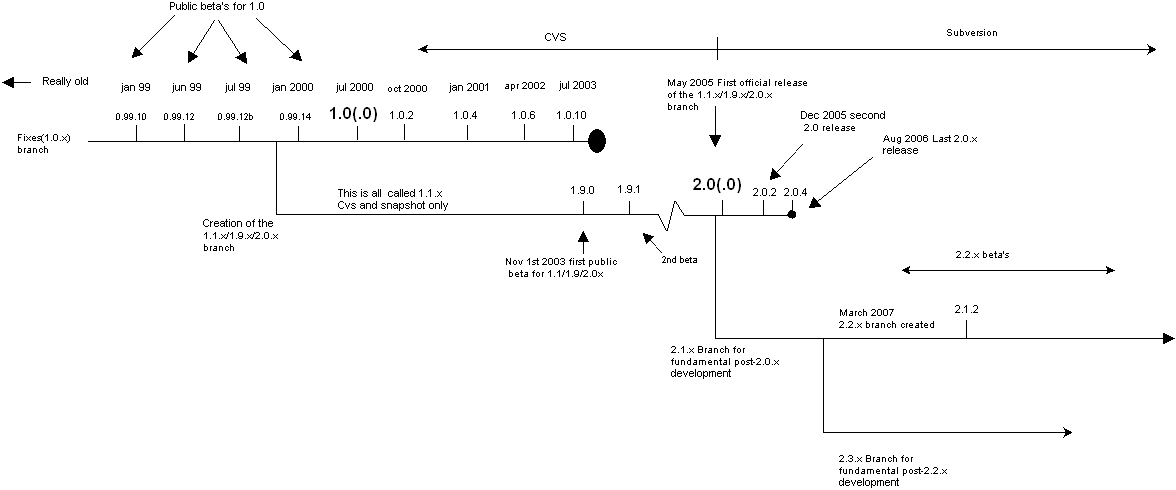
\includegraphics[width=20cm,bb = 0 0 200 100, draft, type=eps]{timeline.png}

While 1.0.x also supports two processors (intel x86 and Motorola m68k).


\section{Requirements\index{Requirements}}

A supported OS and processor are of course the main requirements.
Such info can be better gotten from the website, since the status
changes frequently.\footnote{Actually, while writing this, I witnessed the first working \textquotedblleft Hello
world\textquotedblright{} program on the Sparc V8 architecture :-)} 

The FPC build process needs certain tools. While usually this is all
provided by the OS, or installed by the FPC release package, I name
them here explicitly to make it easier for people to debug build problems. 

The \textbf{main }tools: 
\begin{description}
\item [{ld}] The GNU linker. Links a bunch of .o and .a\textquoteright s
together to form a library (.dll or .so) or a finished program (like
.exe on windows, extensionless on Unix) 
\item [{as}] The GNU assembler. Assembles the textform representation in
a .s or .as file to an .o file. 
\item [{ar}] needed for creating static libraries (.a) from .o\textquoteright s.
Static libraries are used when building for smartlinking. 
\item [{make}] GNU make. Determines the order of what to build. Both on
file as on directory level. Called gmake on {*}BSD 
\item [{ppc386}] or ppc<processor> in general, preferably the last release
version. Bootstrapping from other compilers is not realistic, and,
to my best knowledge, hasn't been attempted in years (1.0.x times)
\end{description}
The first three are found in the package \textquotedblleft binutils\index{binutils}\textquotedblright ,
the version doesn\textquoteright t matter much as long as it is not
a fossil. At least on major platforms. Some platforms package an old
version, e.g. OpenBSD used to package fossils because it still used
a.out as a binary format, though I heard that they finally got rid
of that in version 3.4. These utils are rarely a source of errors,
but depend on the target OS and CPU, which complicates cross-compiling
a bit.

Make is usually obtained from the same source as binutils, but packaged
separately. See the separate section on make below for some common
caveats. 

Windows users that build a system from scratch, should get the makew32.zip
and asldw32.zip (or similar) files from the \textquotedblleft separate\textquotedblright{}
subdirectory of the last release to get the needed external tools. 

Under \emph{Mac OS X/Darwin} , the binutils and make are part of the
Apple developer tools, which for 10.3 are automatically installed
when you install XCode. Fink (an open source software distribution
for Mac OS X) is not strictly required for FPC operation, but most
Unix libraries you might need (like mysql, ncurses etc) are part of
Fink. 


\subsection{ld\index{LD}: The GNU linker. }

The GNU linker is the final step in the building process of a FPC
source to a runnable binary. As said before, a recent version that
supports linkerscript files is the only prerequisite for an easy ride,
except for win32, where the linker should understand \textendash base-file
and \textendash image-base parameters. (these are also already supported
over 3 years though). The supported Win32 platform as far as buildtools
are concerned, is mingw32/64, not cygwin. FPC can link to cygwin libraries
though. 

One could maybe use other linkers then GNU, but that\textquoteright d
require reimplementing the part that calls the linker (this has been
done e.g. for OpenBSD a.out in the 1.0.x compiler and Darwin's mach-O
LD in 2.0+). However keep in mind that the connection between the
assembler and the linker is a common format for the object file (.o).
Changing to a linker that uses a different format might also require
a different assembler, and in turn, a different assembler might require
adaptions to the FPC part that writes the assembler code. However
all these are doable, even for people that aren\textquoteright t complete
compiler wizards. The trouble is often to keep it maintained and used
long enough to become stable.

If your platform is not a mainstream {*}nix or windows, try to find
a linker that supports the \textendash ld-sections\index{-ld-sections}
parameter. The new smartlinking will be based on this LD parameter. 

Starting with FPC 2.1.1, the compiler also has a linker internal for
some platforms which is enabled using -Xi. This internal linker links
way faster, and uses less memory,specially when using smartlinking\footnote{About 250-275 MB as maximum amount of memory used to fully smartlink
Lazarus, as opposed to +/- 1.5GB for GNU LD} . At the time of writing the Windows platforms (PE) are supported
by this internal linker. 


\subsection{as\index{AS}: GNU assembler }

The assembler must be GNU (G)AS, and must be relatively recent. Really
old x86 GNU assemblers might have hidden bugs that don\textquoteright t
surface when used with gcc. Since GNU AS is a typical backend assembler,
in the past addressing modes and opcodes that aren\textquoteright t
emitted by gcc could be problematic. 

An example of this is the OpenBSD 3.x series, where by just substituting
a newer assembler from the ports tree FPC suddenly builds, while it
fails with the packaged assembler. A relatively recent version is
also nice because these probably support newer x86 instructions (SSE2,SSE3).

On some platforms (win32 and x86 ELF), FPC has an internal assembler,
and avoids AS for performance reasons. This internal assembler is
called the binwriter in FPC jargon. The binwriter is a bit more than
a pure assembler though, since it can also directly write static libraries
({*}.a) . While noticeable with ordinary compiles too, the performance
problems that the binwriter solves are mainly noticeable when smartlinking. 

FPC also has the ability to generate code in TASM, NASM, MASM and
WASM (watcom) format. However these aren\textquoteright t frequently
tested, so your mileage may vary. 

On systems that have multiple .o formats (e.g. ARM Endian Little with
its different EABI versions, or platforms where the same assembler
can assemble 32 and 64-bit code depending on a switch) passing extra
parameters to the assembler might be necessary. This can be done by
wrapping the assembler in a shellscript, or using the aswrapper template
in fpcbuild/install/cross.


\subsection{ar\index{AR}: GNU archiver }

The archiver creates archive ( .a) files out of object code files
(.o). This is mainly done to reduce the number of files involved in
the linking process, and on disc. Archive files are often called static
libraries because they contain roughly the same code for static linking
as the .so (or .DLL) files do for dynamic code. (a .dll and .so can
be more than one .o too). The GNU linker can directly access .a libraries. 

AR can be a problem sometimes, since the compiler passes all individual
files on the commandline. Due to e.g. smartlinking and this really
can be a lot, and be larger than the maximal allowed nr of parameters
for the OS. (64k params is too little, 128k is still ok)


\subsection{make\index{make}: GNU make }

The build process of Free Pascal uses plain (GNU make) makefiles that
are generated by \index{FPCMAKE}FPCmake. FPCmake generates the Makefiles
from a global template and the Makefile.fpc in each directory. This
Makefile.fpc is a simple INI file that extends and parameterises the
global template\footnote{which can be found in fpc/utils/fpcm/fpcmake.ini }.
There are plans for the future to get rid of the MAKE utility all
together and replace it with a more specialised own version, but these
are still in the initial stages. The current system is also quite
nice and flexible. 

The currently used make is GNU make, it\textquoteright s available
for nearly all platforms. However there are some platform specific
oddities listed below.
\begin{description}
\item [{Linux}] The only without much oddities. Of all Unices, Linux uses
relatively a lot GNU tools, and less tools descending from the original
unix. If there is a make or make-package on Linux it is most likely
GNU. 
\item [{{*}BSD}] The default make is a pmake variant which is slightly
different from GNU's. The makefile template used by FPC isn\textquoteright t
compatible with pmake at this moment. (hint, hint) GNU make is installable
from the ports tree, usually as devel/gmake\index{gmake}. Don\textquoteright t
forget to put the bin directory of the ports-\$PREFIX (/usr/local/bin,
/usr/pkg/bin etc) into your path, and substitute all use of make by
\textquotedblleft gmake\textquotedblright . In practice this is no
big problem, since gmake is generally available on BSD systems, installed
as dependency of a lot of development related packages.
\item [{BeOS}] On my installation (BeOS 5 Personal Edition) both binutils
and GNU make came with the developer kit. 
\item [{OS/2}] I honestly don\textquoteright t know. There are EMX and
native versions, and of course dos also. Afaik FPC used to be EMX
based, but is currently gearing towards native. I\textquoteright ll
have to research this myself first :-) 
\item [{Dos/Go32V2\index{Go32V2}}] Uses DJGPP Go32V2 utilities. This because
FPC uses the go32v2 extender, and for safe nesting of programs using
an extender, all extenders have to be the same. Including the utils
:-) 
\item [{Netware}] Not even an idea. I never saw this port operational. 
\item [{win32\index{win32}/win64\index{win64}}] Use the mingw set, and
preferably the one distributed with the most recent FPC release. See
below. 
\item [{wince}] My experiences are limited to CE as crosscompilation target.
Some people have e.g. NAS boxes that might allow bootstrap FPC on
a WinCE based host.
\item [{Mac}] OS X Come with Apple Developer tools (which are installed
with XCode on 10.3). Using generic Unix libraries like mysql, ncurses,
postgresql etc might require FINK. 
\end{description}
The situation on win32 often confuses people. This mainly because
there are at least three available sets of the above utils (ar,ld,as,make)
that run on Windows. Any mixing (one util from one category, one from
the other) can also lead to unpredictable results. Anyway, the three
candidates are: 
\begin{description}
\item [{Mingw\index{Mingw}}] (sometimes called mingw32) which is the one
to use. Win32 native tools with a real win32 feel. (driveletters and
backslashes in paths etc) Preferably versions distributed with FPC
releases, since they might include FPC specific critical patches.
E.g. at a certain point it turned out that mingw tools only searched
for a capitalised PATH variable, and not one spelled like \textquotedblleft Path\textquotedblright{}
which is common on NT based Windows versions. See the win32 specific
part of the FAQ on the FPC website for more info. 
\item [{\index{Cygwin}Cygwin}] provides maximal compatibility with Unix,
and can be seen as a Unix compatibility layer. FPC however is really
native on windows, and having half a windows, and half a (compatibility)
unix build system is hard to maintain. FPC does compile with a current
Cygwin install though, but the resulting compiler is no cygwin program.
Also cygwin programs need cygwin1.dll in the correct version . Note
: FPC can link to cygwin, however doesn\textquoteright t need it for
operation (except for the textmode IDE). Recently, Cygwin improved
in native path support, if the paths are fully qualified. Mingw is
still better, but cygwin is usable for emergency operation. 
\item [{go32v2\index{go32v2}}] Go32v2 is dos based, and used via the dos
compatibility system of Windows, don\textquoteright t use it with
the win32 compiler, it would be like using the win32 tools via Wine
on Linux :-) 
\end{description}
A common problem I encountered on win32 is putting the cygwin \textquotedblleft bin\textquotedblright{}
directory in the win32 search path. The mingw make.exe finds the cygwin
shell, and tries to execute certain programs with it. Cygwin has improved
a lot recently though, and currently this seems to work again, at
least if everything is situated on one drive (one can recompile FPC
with only cygwin and a FPC commandline compiler). 

Note that some other development tools (Borland, Microsoft, java)
might also package a make version. Always put FPC as the first directory
in the PATH. 

Due to some new developments with parallel compiling using the FPC
makefiles, \textbf{make 3.80 is strongly recommended as of FPC 2.1.1
(januari 2007 and later)}\emph{.} Unix people with dual cores and
up to date source trees might want to try \textquotedblleft \index{make -j 2}make
-j 2\textquotedblright .


\subsection{FPC itself. ppc386, ppcppc, ppcsparc, fpc. }

Free Pascal is written primarily in itself, in the Pascal dialects
it supports. This has some consequences for beginning the bootstraps. 
\begin{itemize}
\item A normal build of FPC is pretty much only doable with FPC as starting
compiler.
\item Bootstrapping from Delphi was possible for a while under certain circumstances,
but required more skill than plain fpc based bootstrapping, since
the make- files don\textquoteright t support it. Delphi compatibility
has been neglected, since too many Delphi bugs and versioning issues
popped up, and keeping it compilable was a problem. Somewhere between
1.9.4 and 1.9.6 most Delphi workarounds were removed. Newer versions,
starting with D2005 were never tested. The possibility with Delphi
as starting compiler probably failed because while Delphi would have
been great from an availability point, it was easier to use FPC because
of the permanent state of Delphi\textquoteright s bugs, and the large
number of versions in use. 
\item Bootstrapping from TP should possible for 1.0.x versions and earlier.
1.1.x uses delphi classes. However post 0.99.8, already quite some
mastership was required for this to work, since the compiler is a
large program, and the single data segment limitation of TP was a
severe limitation require all kinds of special defines to keep the
size down (which had to be regularly re-evaluated)
\item Bootstrapping from GNU GPC or p2c is not doable. Their TP modi are
not even close to being TP/BP compatible enough, and FPC 1.1.x and
beyond need Delphi compatibility. 
\item Bootstrapping though VP might be doable in theory, at least for 1.0.x
with some considerable skill. This has never been tested though, since
FPC is better on nearly all platforms anyway for basic recompilation,
and less buggy. 
\end{itemize}
The reasons for these choices belong in an advocacy document rather
than here.\footnote{The FAQ lists some reasons, but IMHO not all. }

However practically there is one major disadvantage: you need FPC
to build FPC, and one major advantage: FPC generally needs much less
tools installed to build, compared to e.g. a GCC build. One also needs\textbf{
only }a suitable\textbf{ compiler binary} to bootstrap FPC, not even
a fully fledged FPC installation. (on platforms that don\textquoteright t
come with it, you need the GNU build tools though, see paragraphs
above), and there are essentially \textbf{no library requirements}. 

With the internal linker, in time even the GNU tool requirements may
disappear, allowing a single compiler binary to fully bootstrap the
whole FPC/Lazarus project. 

The file you need to start an ordinary snapshot build is \textquotedblleft ppc<processor>\textquotedblright ,
so ppc386\index{ppc386} for x86, ppcppc for PowerPC. ppcsparc\index{ppcsparc}
for Sun Sparc V8 systems, ppcx64\index{ppcx64} for x86\_64\index{x8664@x86\_64}
(64-bit x86) etc. Till now these files always have been statically
linked. so there is only one Linux/x86 compiler, one FreeBSD compiler
etc. Kernel, library and distribution versions don\textquoteright t
matter. (except maybe major kernel changes in extreme, rare cases
like Linux 1.0.x to 2.0.x) 

For crossbuilds to the same processor but a different OS you don\textquoteright t
need a special cross-compiler\footnote{Assuming the target platform is established. For bleeding edge targets,
ask on the fpc-devel mailing list}. Only for crossbuilding to different processors you\textquoteright ll
need a different one.

Besides this, there is the \textquotedblleft{} \textbf{fpc}\index{fpc(binary)}\textquotedblright{}
binary. This is a common frontend to all ppc<cpu> compilers on a system,
one that compiles for the current architecture and one that compiles
for the rest. The reason for this is that one can use one binary,
and specify the processor with -P. So 
\begin{lyxcode}
fpc~-Ppowerpc~compileme.pp~
\end{lyxcode}
will compile \textquotedblleft compileme.pp\textquotedblright{} using
the PowerPC (ppcppc\index{ppcppc}) compiler if everything is set
up correctly. But we\textquoteright ll get into that later :-) 

The fpc binary can also be used to set compiler version: 
\begin{lyxcode}
fpc~-V1.0~compileme.pp~
\end{lyxcode}
will execute the default compiler (ppc<current processor>) with -1.0
suffixed. Combining with -P is possible. fpc -Ppowerpc -V1.0 will
try to run a binary ppcppc-1.0 as the real compiler. Specially on
Unix this is nice, since only a couple of symlinks allow to switch
versions easily. 

Combined with a masterfully created fpc.cfg file one can build very
powerful crosscompiling systems that autoselect the right targets.
We\textquoteright ll get to that later. 


\subsection{Other external tools}

Sometimes there are other platform dependant tools. Most notably the
Windows resource compiler windres to compiler resourcescripts ({*}.rc)
and dlltool to generate importlibs for FPC generated DLLs so that
certain other compilers (MSVC, mingw) can use them.


\subsection{Other FPC internal tools}

\textbf{Other} tools you might occasionally need:
\begin{description}
\item [{fpcres}] the resource compiler
\item [{data2inc}] A tool to convert various input formats to includefiles.
Usually used for binary to .inc conversion. 
\item [{fpcmake}] A tool to generate makefiles (basically expands Makefile.fpc
to Makefile using a built-in template). In case of problems pass FPCMAKE=(g)echo
to disable it
\item [{fpmake,fppkg}] see separate paragraph (t.b.d)
\end{description}
These tools are not strictly necessary, but the makefiles will invoke
them if timestamps of certain files are corrupted, and the original
is newer than the generated .inc or res file. Touching the xx.inc
file with a touch util can help.


\section{Obtaining source }


\subsection{Introduction }

Right after the FPC 2.0 release, the FPC project change to use SVN
as source version management system, for reasons mostly related to
merging and branching. 

Usually when building a snapshot, the source is obtained via SVN,
and comes as a large source tree with fpc/ as the root directory of
the repository. However the source is usually also downloadable as
an archive from the main site\footnote{\textbackslash{}href\{ftp://ftp.freepascal.org/pub/fpc/snapshot/v26/source/fpc.zip\}\{ftp://ftp.freepascal.org/pub/fpc/snapshot/v26/source/fpc.zip
(2.6.x)\}}\footnote{\textbackslash{}href\{ftp://ftp.freepascal.org/pub/fpc/snapshot/v27/source/fpc.zip\}\{ftp://ftp.freepascal.org/pub/fpc/snapshot/v27/source/fpc.zip
(2.7.x development series)\}}. This archive is getting larger each month though, and is already
25M zipped.

A better way is to get the sources via SVN, which allows to upgrade
sources to more recent versions incrementally. (i.o.w. the second
time, it only downloads changes)


\subsection{SVN Modules}

The FPC and Lazarus source is spread out over several SVN modules:

\begin{tabular}{|l|l|}
\hline 
{\small{}Module } & {\small{}Description}\tabularnewline
\hline 
\hline 
{\small{}fpc} & {\small{}The core FPC repository. Contains compiler, RTL, textmode
IDE and most non visual libraries }\tabularnewline
\hline 
{\small{}fpcdocs} & {\small{}The FPC documentation source (in \LaTeX and fpdoc XML format)}\tabularnewline
\hline 
{\small{}fpcprojects} & {\small{}Projects not yet suitable for distribution together with
FPC are parked here. (includes IRC bot)}\tabularnewline
\hline 
{\small{}fpcbuild} & {\small{}Contains fpc and fpdocs tree as well as the install and demo
dirs and a makefile for release packaging.}\tabularnewline
\hline 
{\small{}lazarus } & {\small{}The Lazarus project (visual classes library LCL and the Lazarus
IDE/RAD)}\tabularnewline
\hline 
\end{tabular}


\subsection{Downloading source via SVN }

To check out\index{Checkout(SVN)} a module, use the follow line:
\begin{lyxcode}
svn~co~http://svn.freepascal.org/svn/<module>/trunk~<module>~

\#

\#~Examples:~

\#~

\#~FPC~

\#~svn~co~http://svn.freepascal.org/svn/fpc/trunk~fpc~

\#~

\#~fpcdocs~

\#~

svn~co~http://svn.freepascal.org/svn/fpcdocs/trunk~fpcdocs~

\#~

\#~fpcprojects~(has~no~branches,~maybe~you~don't~need~/trunk~at~the~end)~

\#~

svn~co~http://svn.freepascal.org/svn/fpcprojects/trunk~fpcprojects~

\#~

\#~lazarus~

\#~

svn~co~http://svn.freepascal.org/svn/lazarus/trunk~lazarus~
\end{lyxcode}
To check out a branch, replace \textquotedblleft trunk\textquotedblright{}
in the above lines with the branches/<branch name>. E.g. to check
out the branch fixes\_2\_6: 
\begin{lyxcode}
svn~co~http://svn.freepascal.org/svn/fpc/branches/fixes\_2\_6~fpc-2.6.x~
\end{lyxcode}
Specific releases are tagged with a tag that is formated like \index{RELEASE222@RELEASE\_2\_2\_2}RELEASE\_2\_6\_0
, and can be checked out like this: 
\begin{lyxcode}
svn~co~http://svn.freepascal.org/svn/fpc/tags/RELEASE\_2\_6\_0~fpc-2.6.0
\end{lyxcode}

\subsection{Updating\index{Updating(SVN)} the source via SVN }

The advantage of getting source via SVN is of course the incremental
updating. This is very simple with SVN, simply use \textquotedblleft svn
up x\textquotedblright , if x is a directory where you have checked
out something before. http path, fixes and branches are automatically
read from the system. 

Examples: 
\begin{lyxcode}
svn~up~fpc~

\#~

svn~up~fpc-2.6.0
\end{lyxcode}

\subsection{Reverting\index{Reverting(SVN)} SVN checkouts }

Something new in SVN is reverting. If local edits cause conflicts
when updating your checkout, or if you want to be 100\% sure that
there are no local edits, you should revert your checkout, to make
sure that your local copy is really in sync with the SVN server. 

You should do this if you\textquoteright re having a problem that
other people on IRC and mailing lists can\textquoteright t duplicate,
and your starting compiler is correct. 

Examples: 
\begin{lyxcode}
svn~revert~-R~fpc~
\end{lyxcode}

\subsection{Exporting\index{Exporting(svn)} (win32/64 users, read this!) }

Exporting is basically retrieving a local working copy from a checkout.
Typical reasons to build in an export instead of a checkout are: 
\begin{itemize}
\item You are doing a release build. E.g. making RPMs, debs, freebsd ports
entries etc. 
\item You are building on win32 , and want to use \textquotedblleft make
install\textquotedblright{} to install the build, AND you want to
install examples.
\end{itemize}
The problem on windows is that some tools get confused by the read-only
attributes set on administrative files by some SVN clients. Since
svn export only copies the repository\textquoteright s content, and
not the administrative files, this is a good workaround. Exporting
is effectively copying, so this workaround takes about the same time
and space as manually copying the checkout. 

The format of the export command is: 
\begin{lyxcode}
svn~export~path\textbackslash{}to\textbackslash{}checkout~exportdirectory~
\end{lyxcode}
Example: 
\begin{lyxcode}
svn~export~d:\textbackslash{}fpc~fpcexport~

or~

svn~export~/usr/local/src/fpc~fpc~
\end{lyxcode}
If the second argument already exists, SVN will refuse to do this.
In that case use \textendash force to force svn to update. 

\textbf{Not}e 1: I haven\textquoteright t tested this yet, but cleaning
the repository before exporting could speed up somewhat, specially
on windows.

Note 2: For a \textbf{faster solution} see the build tricks section.


\subsection{(dist)Clean before update}

In general a FPC repository should clean the files it generates. However
when tracking branches, the files that are generated might vary, and
already built files may not be removed, since they belong to units
deleted or moved in the new revision.

Therefore it is generally better to first call ``make distclean''
before updating the repository.


\subsection{More info about SVN }

More info about FPC and SVN can be found here \href{http://www.freepascal.org/wiki/index.php/SVN\_Migration}{http://www.freepascal.org/wiki/index.php/SVN\_Migration}


\section{Extension\index{Extensions (file-)} conventions }

FPC defines some extensions that need some clarification: 
\begin{description}
\item [{.o}] The actual code of a compiled unit or main program 
\item [{.a}] The actual code of a compiled unit or main program when smartlinking. 
\item [{.ppu}] The rest of the compiled unit that is not actual code. (like
information about directives that where defined when compiling, the
parsed interface etc) 
\item [{.s}] Assembler code (to be assembled .o) generated by the compiler. 
\item [{.as}] Assembler code in source form (there never was a pascal equivalent).
Usually program startup code. 
\item [{.s}] files. .rst resourcestring files for internationalisation. 
\item [{.\$\$\$}] temporary files. Can be safely removed usually 
\item [{.res}] Windows or OS/2 resource file 
\item [{link.res}] Linker script file. Contains which files make up the
binary, and what external libraries are used. NOT a windows resource
file.
\item [{ppas.sh}] (or .bat) batchfile that calls the linker with the correct
arguments. 
\item [{{*}.lrs}] Lazarus resources, old style
\item [{{*}.rc}] Resource source file, to be processed by windres to .res
\end{description}
\footnote{The extensions on win32 originally ended in ``w'' ({*}.ow, {*}.ppw),
which was done to avoid confusion with dos compilers on the same system.
However this has been superceded by a better directory structure which
was needed for easy crosscompiling, and in the 1.1.x/1.9.x branch
the extensions for win32 are renamed back to .ppu/.a/.o }

So in the FPC distribution you will find a .ppu, an .a and an .o per
compiled unit.


\section{\index{Directory layout}Directory layout \label{sec:Directory_layout}}

Essentially the FPC layout is quite flexible. The binary (ppc386,
ppc68k or ppcppc) must be able to find a configuration file, and that
file can then specify the rest of the configuration. So the layouts
described here are the default layouts as installed by the releases.
Some, like the Dos (go32v2) port have a simpler layout, due to platform
limitations.

The base installation of FPC has these main categories: 
\begin{description}
\item [{binaries}] The base binaries (fpc, ppc68k, ppcppc, ppcsparc, ppcarm
and ppcx64) must be in the search PATH of the OS. If you execute fpc,
fpc must be able to find the other ones (ppcppc, ppc386 etc), also
via the PATH. 
\item [{\index{fpc.cfg}fpc.cfg}] The binary must be able to find the configuration
file in one of the default locations as specified for that OS. (see
platform dependant sections) 
\item [{units}] The configuration file must define the correct path to
the RTL and other packages compiled for that platform and cpu. This
is usually a tree. Crosscompile units also belong in this tree. 
\item [{help}] In future versions, this will be the directory where the
CHM files for the textmode IDE reside.
\item [{doc}] documentation (pdf)
\item [{doc-html}] documentation html, can also double as help for textmode
IDE.
\item [{(binutils)}] The binutils (LD,AS,AR) have to be in the PATH, or
their directory should be specified in the fpc.cfg file or on the
commandline with the -FD parameter. On operating systems that don\textquoteright t
install the binutils by default, these are installed by the FPC installation
process in the same directory as the main binaries, so this is usually
not a problem when not crosscompiling or mixing two FPC installations
(e.g. a DOS and Windows installation on one machine). Note that specifying
in the fpc.cfg file only works when compiling programs by hand. When
compiling a new compiler, the fpc.cfg file is ignored by the makefile.
\end{description}
Besides these there are source tree, documentation,the compiler localisation
(language) and example directories. However these are only interesting
for real release distribution engineering,and don\textquoteright t
influence the workings of the compiler itself. This because the compiler
has the source already in compiled form in the .o, .a and .ppu files
in the units directory. The place of the source doesn\textquoteright t
really matter. The only thing that needs the source directory for
automated processing is lazarus, and one can enter any path in Lazarus\textquoteright{}
FPC source dialogue. 

When writing paths in fpc.cfg, some substitutions are automatically
done, e.g. 
\begin{description}
\item [{\$FPCTARGET\index{FPCTARGET@\$FPCTARGET}}] is replaced by the
architecture - operating system combination you are compiling for.
(e.g. i386-linux) 
\item [{\$FPCVERSION\index{FPCVERSION@\$FPCVERSION}}] is replaced by the
version of the FPC compiler reading it, and finally 
\item [{\$FPCCPU\index{FPCCPU@\$FPCCPU}}] is replaced by the processor
which the compiler is targeting. 
\item [{\$FPCOS\index{FPCOS@\$FPCOS}}] is replaced by the operating system. 
\item [{\$FPCFULLVERSION\index{FPCFULLVERSION@\$FPCFULLVERSION}}] is replaced
by a compiler version with an extra patchlevel. (2.4.x+) 
\item [{\$FPCDATE\index{FPCDATE@\$FPCDATE}}] is replaced by the current
date.
\end{description}
Since filesystems hierarchies differ with the OS, I\textquoteright ll
put some OS specific information in the following sections.


\subsection{Unix (and full clones like Linux) \label{sub:unix dir layout}}

Under Unix, most directories are relative to the so called prefix.
A prefix is a kind of root directory for package installing. Common
prefixes are /usr, /usr/local, /usr/exp and /usr/pkg (the last one
is common on NetBSD). 

The usual convention is that programs that come with the base-distribution
go into /usr, and hand-compiled or hand-installed packages go to /usr/local.
However the definition of base-distribution varies with the distribution
and OS. The main idea is to give root (the administrator) trusted
users the ability to install and manage less important packages in
/usr/local while keeping the base system only writable for the administrator
(group) himself. Linux distributions are traditionally more likely
to install packages into /usr instead of /usr/local, but not every
distribution does that. \textquotedblleft man hier\textquotedblright{}
should list some of the conventions used on your Unix version.

If directories are relative to a prefix, they are noted as \$PREFIX/the/rest/of/the
path. Note that this has nothing to do with \$FPC<x> substitutions
in fpc.cfg. \$PREFIX is shellscript notation for \textquotedblleft get
content of environment variable PREFIX\textquotedblright . Compiled
units go into \$PREFIX/fpc/\$FPCVERSION/units/\$FPCTARGET. Units used
for crosscompiling also go into \$PREFIX/fpc/\$FPCVERSION/units/\$FPCTARGET.

Binaries go into directory \$PREFIX/bin, however sometimes these are
only symlinks to the actual files in \$PREFIX/lib/fpc/\$FPCVERSION
directory to easily switch versions. Since the binary can find its
own unit files using versioned info in fpc.cfg when properly set up,
usually the default binary is the only thing that needs to be swapped. 

The place where configuration files are searched on unix are: /etc/fpc.cfg,
\textasciitilde{}/.fpc.cfg. \$PREFIX/etc/fpc.cfg is searched from
1.9.8 onwards. (note; \textasciitilde{} means home directory on Unix)

So let\textquoteright s take \$PREFIX=/usr/local, \$VERSION=2.6.0,
\$FPCCPU=i386, \$FPCOS=freebsd and \$FPCTARGET=i386-freebsd as an
example, and see what file goes where:

\begin{tabular}{|l|l|l|}
\hline 
{\small{}File(s)} & {\small{}location } & {\small{}remarks}\tabularnewline
\hline 
\hline 
{\small{}fpc} & {\small{}/usr/local/bin} & \tabularnewline
\hline 
{\small{}ppc386} & {\small{}/usr/local/bin} & {\small{}actually symlinked to /usr/local/lib/fpc/2.6.0/ppc386}\tabularnewline
\hline 
{\small{}ppcppc} & {\small{}/usr/local/bin} & {\small{}actually symlinked to /usr/local/lib/fpc/2.6.0/ppcppc}\tabularnewline
\hline 
{\small{}rtl for i386-freebsd} & {\small{}/usr/local/lib/fpc/2.6.0/units/i386-freebsd/rtl} & \tabularnewline
\hline 
{\small{}rtl for i386-linux} & {\small{}/usr/local/lib/fpc/2.6.0/units/i386-linux/rtl } & {\small{}(cross operating system compiling)}\tabularnewline
\hline 
{\small{}rtl for powerpc-netbsd} & {\small{}/usr/local/lib/fpc/2.6.0/units/powerpc-netbsd/rtl} & {\small{}(cross architecture and OS compiling, endianness) }\tabularnewline
\hline 
{\small{}rtl for x86\_64-win64} & {\small{}/usr/local/lib/fpc/2.6.0/units/x86\_64-win64/rtl} & {\small{}(cross arch, OS, wordsize)}\tabularnewline
\hline 
\end{tabular}


\subsection{Windows and Dos }

The windows and dos case is pretty much the same. Except that \$FPCTARGET=i386-win32
for windows, and \$FPCTARGET=i386-go32v2 for dos.\textbf{ It is advised
to avoid using spaces in directory names. While (win32) fpc can handle
it, some versions of the binutils and other tools can not (yet), or
need carefully placed quotes. }

Both these two OSes have a specific directory with all FPC related
files (including the documentation etc) in them, default is usually
used to be c:\textbackslash{}pp, but has been changed to c:\textbackslash{}fpc\textbackslash{}2.4.0
since 2.0. I call this path \$INSTALLDIR. Usually there aren\textquoteright t
other versions in the same \$INSTALLDIR A different version means
a different \$INSTALLDIR, at least in the default situation. 

All binaries go into \$INSTALLDIR\textbackslash{}bin\textbackslash{}\$FPCTARGET.
This directory should be in the PATH. This directory is quite full,
since there are other tools and utilities installed. However if the
target is marked to require 8.3 compatible naming (Go32v2, OS/2),
the binary path is not \$FPCTARGET (e.g. bin/i386-go32v2) but just
\$FPCOS (e.g. bin/go32v2).

Compiled units go into \$INSTALLDIR\textbackslash{}units\textbackslash{}\$FPCTARGET
and deeper, at least under 2.0+. 

Configuration files are searched in the same directory as the binary
(\$INSTALLDIR\textbackslash{}bin\textbackslash{}\$FPCTARGET), but
if a environment variable HOME exists also in \%HOME\%/.fpc.cfg.

So let\textquoteright s assume \$INSTALLDIR=c:\textbackslash{}fpc\textbackslash{}2.6.0
and the default \$FPCTARGET=win32 

\begin{tabular}{|l|l|l|}
\hline 
{\small{}File(s)} & {\small{}location } & {\small{}remarks}\tabularnewline
\hline 
\hline 
{\small{}fpc} & {\small{}c:\textbackslash{}fpc\textbackslash{}2.6.0\textbackslash{}bin\textbackslash{}i386-win32} & \tabularnewline
\hline 
{\small{}ppc386} & {\small{}c:\textbackslash{}fpc\textbackslash{}2.6.0\textbackslash{}bin\textbackslash{}i386-win32} & \tabularnewline
\hline 
{\small{}ppcrossppc} & {\small{}c:\textbackslash{}fpc\textbackslash{}2.6.0\textbackslash{}bin\textbackslash{}i386-win32} & \tabularnewline
\hline 
{\small{}rtl for i386-win32} & {\small{}c:\textbackslash{}fpc\textbackslash{}2.6.0\textbackslash{}units\textbackslash{}i386-win32\textbackslash{}rtl} & {\small{}(cross architecture and OS compiling) }\tabularnewline
\hline 
{\small{}rtl for i386-linux} & {\small{}c:\textbackslash{}fpc\textbackslash{}2.6.0\textbackslash{}units\textbackslash{}i386-linux\textbackslash{}rtl} & {\small{}(cross operating system compiling)}\tabularnewline
\hline 
{\small{}rtl for powerpc-netbsd} & {\small{}c:\textbackslash{}fpc\textbackslash{}2.6.0\textbackslash{}units\textbackslash{}powerpc-netbsd\textbackslash{}rtl} & \tabularnewline
\hline 
{\small{}rtl for x86\_64-win64} & {\small{}c:\textbackslash{}fpc\textbackslash{}2.6.0\textbackslash{}units\textbackslash{}x86\_64-win64/\textbackslash{}rtl} & \tabularnewline
\hline 
\hline 
{\small{}Cross binutils} & {\small{}c:\textbackslash{}fpc\textbackslash{}2.6.0\textbackslash{}cross} & {\small{}(not installed by default setup) }\tabularnewline
\hline 
\hline 
{\small{}libs for i386-win32} & {\small{}c:\textbackslash{}fpc\textbackslash{}2.6.0\textbackslash{}libs\textbackslash{}i386-win32} & {\small{}(not installed by default setup) }\tabularnewline
\hline 
\hline 
{\small{}libs for i386-linux} & {\small{}c:\textbackslash{}fpc\textbackslash{}2.6.0\textbackslash{}libs\textbackslash{}i386-linux} & {\small{}(not installed by default setup) }\tabularnewline
\hline 
\end{tabular}


\subsection{Where are my units? }

Starting with later versions of FPC 1.9.5, the fpc makefiles create
a directory to store the created units. The main reason for this is
building for multiple targets without cleaning in between. 

So when just build (not installed), the rtl units files are in fpc/rtl/freebsd/units/\$FPCTARGET.
This is a silly example of course, since the RTL is platform specific,
but this change is systematic, so for the RTL too.


\section{The fpc.cfg\index{cfg} configuration file }

\textbf{Note: }Former versions used \index{ppc386.cfg}ppc386.cfg
as configuration file. Even latere 1.0.x versions already support
fpc.cfg. In time ppc386.cfg will be dropped, so \emph{please} use
fpc.cfg.

A correct configuration file should at least do the follow things: 
\begin{enumerate}
\item ( \textbf{most important }) Provide the place where to find the correct
precompiled units for the current selected operating system and architecture.
In IDE\textquoteright s this option is usually called UNITPATH\index{UNITPATH}
Option:\textbf{ -Fu\index{-Fu} }
\item If other binutils then for the default platform need to be used (like
in the case of crosscompiling), then fpc.cfg should allow the compiler
to find them. I don\textquoteright t know what name IDE\textquoteright s
typically use for this, but BINUTILS PATH\index{BINUTILS PATH} or
GNU UTILS PATH would be appropriate Option: \textbf{-FD\index{-FD}} 
\item Extra paths where static and shared libraries are searched. Often
called library path Option: \textbf{-Fl\index{-Fl} }
\item ( minor ) By default the compiler shows only very little errors, warnings
and information. It\textquoteright s convenient to add some verbosity
parameters to fpc.cfg. Option \textbf{-vihw -l}. \footnote{The warning system is currently being expanded to have more flexibility. }
\item (crosscompiling) Binutils for cross compiling are often prefix with
cpu-operatingsystem(e.g. i686-ming32),this prefix can be specified
using -XP<prefix> parameter, or using makefiles using BINUTILSPREFIX\index{BINUTILSPREFIX}.
Option \textbf{-XP\index{-XP}} 
\end{enumerate}
There are other interesting possibilities of fpc.cfg, (like internationalised
errormessages, setting the compiler in a different mode per default,
always to try smartlinking etc) but these are the important ones for
normal development.

\textbf{Note: }Keep in mind that when using the makefiles supplied
with the FPC source, the fpc.cfg is \textbf{NOT} read. This is to
avoid problems with two RTLs, the old and the new one, when bootstrapping
the system.


\subsection{Unit path -Fu\index{-Fu} }

The -Fu case is pretty much as described in the directory layout paragraphs
(\ref{sec:Directory_layout}), there are two things in which the -Fu
compiler option differs from the directory layout as described before.
If I append an asterisk ({*}) to a path, it means that it should search
all directories below that directory too, and that the layout for
crosscompiled units is a bit different.

We can use the directive \index{FPCCROSSCOMPILING@FPC\_CROSSCOMPILING}FPC\_CROSSCOMPILING
to detect crosscompilation. The FPC manual has a list of other defines
that can be tested.

\textbf{Unix:} If we assume that the compiler is installed to PREFIX
/usr/local, and we are using FreeBSD/i386 as host OS, this becomes: 
\begin{lyxcode}
\#~This~is~pretty~generic~for~OSes~with~{*}nix~filesystem~layout~

-Fu/usr/local/lib/fpc/\$FPCVERSION/units/\$FPCtarget/{*}~

\#....or~suitable~for~crosscompiling.~Note~that~the~/cross/~dir~is~not~necessary~

\#~and~only~added~as~example.~

\#ifdef~FPC\_CROSSCOMPILING

\#~OS~not~default~->~CROSS~

-Fu/usr/local/lib/fpc/\$FPCversion/cross/\$fpctarget/units/{*}~

\#else~

~\#ifndef~cpu86\index{cpu86}~

~\#~Processor~not~default~->~CROSS~

~~-Fu/usr/local/lib/fpc/\$FPCversion/cross/\$fpctarget/units/{*}~

~\#else~

~~-Fu/usr/local/lib/fpc/\$FPCVERSION/units/\$FPCtarget/{*}~

~\#endif~

\#endif~
\end{lyxcode}
Win32 and Dos installed in c:\textbackslash{}fpc\textbackslash{}2.4.0 
\begin{lyxcode}
-Fuc:\textbackslash{}fpc\textbackslash{}2.4.0\textbackslash{}units\textbackslash{}\$FPCtarget\textbackslash{}{*}~

\#~or~suitable~for~crosscompiling~

\#~OS~not~default~->~CROSS~

-Fuc:\textbackslash{}fpc\textbackslash{}2.4.0\textbackslash{}units\textbackslash{}\$fpctarget\textbackslash{}{*}~

\#~win32~binutils~are~in~the~path~

\#ifndef~win32~

\#~set~path~to~crossutils.~Assuming~in~one~dir.~

-FDc:\textbackslash{}fpc\textbackslash{}2.4.0\textbackslash{}bin\textbackslash{}cross~

\#~this~is~not~100\%~safe.~GNU~and~FPC~target~naming~differ~

-XP\$FPCTARGET-~

\#endif~
\end{lyxcode}
Keep in mind that extra paths (e.g. for own custom packages) can be
added. There is also no reason not to use \$FPCVERSION in the win32
case. It is just an example.


\subsection{Binutils path -FD\index{-FD} }

The problems with binutils 
\begin{enumerate}
\item We only have to set -FD if we set up for crosscompiling. Either when
cross compiling to a different processor or a different OS. So we
have to determine default OS and CPU somehow.
\item Under Unix, there are usually specific dirs for crossutils, but the
exact place and name differs with version. Win32 doesn\textquoteright t
have something like that at all. For win32 I propose an example layout
as described above. 
\item FPC and GNU platform naming differ
\end{enumerate}
\textbf{Unix} : As an example I take FreeBSD on an ordinary PC. The
location below (/usr/local/processor-operatingsystem) is where the
binutils base distribution installs cross compiled utils by default
under FreeBSD. However sometimes how FPC names an OS can differ from
how the binutils name it. In that case you have to be more verbose,
which I have done for the case of crosscompiling to windows\footnote{{\small{}Lazy people simply would make a symlink from the fpc naming
to the binutils naming. However being lazy is not allowed for tutorial
writers.}} . 

So our configuration file becomes: 
\begin{lyxcode}
\#ifdef~FPC\_CROSSCOMPILING\index{FPCCROSSCOMPILING@FPC\_CROSSCOMPILING}

\#~other~binutils~if~OS~differs~

\#ifdef~win32~

\#~win32~is~an~exception~

\#~FPC~OS~name~:~win32~Binutils~OS~name~:~mingw32~

\#~FPC~processor:~i386~Binutils~processor:~i686~

-FD/usr/local/i686-unknown-mingw32/bin~

\#else~\#~we~hope~that~the~fpc~and~binutils~name~match:-)~

-FD/usr/local/\$FPCTARGET/cross~

\#endif~

\#else~

\#ifndef~cpu86~

\#~other~binutils~if~processor~differs~

-FD/usr/local/\$FPCTARGET/cross~

\#endif~\#endif~
\end{lyxcode}
Win32 and Dos: Pretty much the same. However contrary to Unix I haven\textquoteright t
really tested this. Again I assume FPC to be installed in c:\textbackslash{}fpc\textbackslash{}2.4.0
.However the binutils are in d:\textbackslash{}binutils and deeper
and named like under {*}BSD:
\begin{lyxcode}
\#ifndef~win32~

\#~other~binutils~if~OS~differs~

-FDd:\textbackslash{}binutils\textbackslash{}\$FPCTARGET\textbackslash{}bin~

\#else~

\#ifndef~cpu86

\#~other~binutils~if~processor~differs~

-FDd:\textbackslash{}binutils\textbackslash{}\$FPCTARGET\textbackslash{}bin

\#endif~

\#endif~
\end{lyxcode}
\textbf{Using makefiles }

When using makefiles, one can set the -FD parameter by passing CROSSBINDIR\index{crossbindir@CROSSBINDIR}=<path>
to make. This ensures that the parameter is passed correctly from
makefile to makefile (in nested directory hierarchies).


\subsection{Binutils prefix, all binutils in one directory}

A somewhat newer addition is the -XP\index{-XP} parameter which sets
a prefix for all binutils, so if you add \textbf{-XPbla-die-bla-}
to the fpc commandline then all calls to as and ld will be prefixed
with \textbf{bla-die-bla-} . The main reason for this is that by default,
cross compiled binutils are named <cpu>-<target>-<filename>,and not
just <filename>.

When doing a cross snapshot (or cycle), setting the make variable
BINUTILSPREFIX\index{binutilsprefix@BINUTILSPREFIX} will make sure
that -XP is passed on the right moments. 

If we assume the binutils for cross compiling are all in one directory,
the above piece of code becomes:  
\begin{lyxcode}


\#ifdef~FPC\_CROSSCOMPILING

~\#~other~binutils~directory~if~processor~or~target~OS~differs~

~-FD/usr/local/cross/bin~

~\#~set~prefix~to~select~the~right~ones~from~that~directory:~

~-XP\$FPCTARGET-~

~\#endif~


\end{lyxcode}
This assumes that binutils naming of platforms is the same as FPC\textquoteright s.
It isn\textquoteright t however, there are a few exceptions: 

\begin{tabular}{|c|c|c|c|}
\hline 
{\small{}Usual name} & {\small{}FPC name} & {\small{}Binutils name} & {\small{}ppc<x> name}\tabularnewline
\hline 
\hline 
{\small{}(32-bit windows)} & {\small{}win32} & {\small{}cygwin or mingw32} & {\small{}(OS not CPU)}\tabularnewline
\hline 
{\small{}i386 or x86} & {\small{}i386} & {\small{}i386,i486,i586,i686} & {\small{}386}\tabularnewline
\hline 
{\small{}Sunos/Solaris} & {\small{}sunos} & {\small{}solaris} & \tabularnewline
\hline 
{\small{}PowerPC} & {\small{}powerpc} & {\small{}powerpc} & {\small{}ppc}\tabularnewline
\hline 
\end{tabular}

So for these targets we would have to make exceptions. (see e.g. script
code in the fpcbuild/install repository, e.g. samplecfg and install.sh)


\subsection{Library path -Fl\index{-Fl} \index{Library path}}

The library path is where static libraries (and shared libs under
unix) can be found. While this is very important for the Unix platform,
the FPC compiler on windows and dos also can link to GCC (and variants)
libraries, so FPC must be able to find them. 

The library path is of course target and processor dependant. One
couldn\textquoteright t link FreeBSD/x86 libraries to a Linux/Powerpc
binary. So essentially we are doing the same trick as with the unit
path. If the default targets are used, on unix it is set to the default
directories, otherwise it is set to some hierarchy where the user
is supposed to install his cross libraries.

\textbf{Unix} : As an example I take FreeBSD on an ordinary PC, because
most BSDs, specially on ordinary PCs have a \textquotedblleft compatibility\textquotedblright{}
Linux libraryset to run proprietary Linux programs for which no FreeBSD
version exists. This mode is called the Linuxator\footnote{The linuxator\index{linuxator} is strictly speaking an emulator.
However the emulation layer is so thin (a few 10\textquoteright s
of kbs) that there is no noticable performance loss. Since all libs
are in memory twice (Linux+FreeBSD) it eats some extra memory though. }. The Linuxator libs are usually SUSE based and in /compat/linux/
and deeper. NetBSD has a huge set of such emulations. Anyway, here
is the snippet, it assumes the user to build a hierarchy of cross
libs under /usr/local/crosslibs 
\begin{lyxcode}
\#undef~specialoscpu~



\#ifndef~FPC\_CROSSCOMPILING

\#define~specialoscpu~

\#~DEFAULT~

\#~libraries~outside~base~are~installed~with~PREFIX=/usr/local~

-Fl/usr/local/lib~

\#~however~X~stuff~is~installed~with~PREFIX=/usr/X11R6~

-Fl/usr/X11R6/lib~

\#endif~



\#ifdef~linux~

\#ifdef~cpu86~

\#~CROSS,~BUT~SPECIAL,~FreeBSD~optionally~has~a~Linux~userland~on~board~

\#~for~the~linuxator.~Usually~it~is~some~SUSE~version.~

\#define~specialoscpu~

-Fl/compat/linux/lib~

-Fl/compat/linux/usr/lib~

-Fl/compat/linux/usr/X11R6/lib~

\#endif~

\#endif~

\#~libraries~not~existing~on~target~by~default.~Reverting~

\#~to~special~cross~directories~

\#ifndef~specialoscpu~

-Fl/usr/local/crosslibs/\$FPCTARGET/lib~

-Fl/usr/local/crosslibs/\$FPCTARGET/usr/lib~

-Fl/usr/local/crosslibs/\$FPCTARGET/usr/local/lib~

-Fl/usr/local/crosslibs/\$FPCTARGET/usr/X11R6/lib~

\#endif~
\end{lyxcode}
\textbf{Win32 and Dos}: Exactly the same idea. Some directory with
the hierarchy (d:\textbackslash{}crosslibs for now), but none as default.
If you have a suitable gcc equivalent (djgpp for dos, cygwin and mingw
for win32), you could add it to the space for the default.
\begin{lyxcode}
\#ifndef~win32~

\#~other~binutils~if~OS~differs~

-Fld:\textbackslash{}crosslibs\textbackslash{}\$FPCTARGET\textbackslash{}lib~

-Fld:\textbackslash{}crosslibs\textbackslash{}\$FPCTARGET\textbackslash{}usr\textbackslash{}lib~

\#etc~

\#else~

\#ifndef~cpu86~

\#~other~binutils~if~processor~differs~

\#~maybe~somebody~does~a~port~for~win32/Sparc~or~so.~

-Fld:\textbackslash{}crosslibs\textbackslash{}\$FPCTARGET\textbackslash{}lib~

-Fld:\textbackslash{}crosslibs\textbackslash{}\$FPCTARGET\textbackslash{}usr\textbackslash{}lib~

\#else~

\#~DEFAULT~

\#endif~

\#endif~
\end{lyxcode}

\subsection{Verbosity options }

Well, there is not much to tell. The default is ok for normal use,
and I never change it in the fpc.cfg (I wrote it down below for completeness),
for more info see the manual. Note that any verbosity setting in fpc.cfg
can be overriden on the commandline (e.g. for debugging, typically
uses -va on the cmdline ) 
\begin{lyxcode}
\#~write~FPC~logo~lines.~

-l~

\#~Display~Info,~Warnings,~Notes~and~Hints~

-viwn~
\end{lyxcode}

\section{The order to compile parts of FPC}

Packages is a bit of an ambiguous term when used in the FPC project\footnote{See alsohttp://wiki.freepascal.org/packages \url{http://wiki.freepascal.org/packages}}.
Sometimes \textquotedblleft packages\textquotedblright{} refers exclusively
to the separate unit sets in the packages/ directory of the source
tree, sometimes it also includes the other separately compilable parts
of the project (like compiler, rtl, fcl, ide, fvision, lazarus, installer
and utils). In this paragraph it\textquoteright s the latter one. 

The directory structure of the packages has been reorganized starting
with FPC 2.2.4. \footnote{This reorganization was made possible with improvements in the fpcmake
system. However in time, the fpcmake system will disappear, and be
replaced with the fpmake/fppkg system that is already included for
testing in 2.2.4+}. Most importantly, the fpcmake system now figures out its own dependencies,
so all packages (including FCL and FV) could move to /fpc/packages.
This great simplifies building and maintenance of the packages. The
units of the FCL were also regrouped into multiple packages.

Of course there iss till a certain sequence one should follow when
building FPC, which is hardcoded in the top Makefile. This because
some packages need other packages and need to be build first. The
usual order is:
\begin{enumerate}
\item bootstrap the compiler (\index{make cycle}make cycle) 3x compiler,
3x rtl 
\item Rebuild the RTL smartlinking 
\item Build the packages directory including the FCL and FV packages.
\item Build the textmode IDE. 
\item utils/ directory including fpcmake in utils/fpcm 
\end{enumerate}
Lazarus can be built after the main build (with or without IDE). However
install the main build \emph{first}. Some directories are not built
at all in a standard build of the fpc repository:
\begin{enumerate}
\item demoes and example directories of packages
\item the regression testing suite (tests/) 
\end{enumerate}
Examples are often compilable by descending into the package directory
and executing ``\index{make examples}make examples''.


\subsection{Some interesting build scripts}

Some of these principles are used in some of the scripts used to build
releases, test crosscompiling etc. 
\begin{itemize}
\item fpc/installl/install.sh is the installer script for unix. Nicely demonstrates
platform name (GNU->FPC) conversion 
\item fpc/install/cross/buildcrossbinutils is a script to mass-build cross
binutils 
\item fpc/install/cross/buildcrosssnapshot is an attempt at building cross
snapshots. Works in principle, however the shared linking of mkxmlrpc
and the textmode IDE are troublesome. 
\item fpc/install/makepack is a release building script. It requires the
target name (i386-linux, i386-win32 etc) as parameter 
\end{itemize}

\section{Smart linking }

Smartlinking (ld/gcc documentation calls it dead code elimination
) essentially means avoiding linking of unused code into the final
binary. 

The problem is that the GNU linker can do dead code elimination, but
usually (read: with gcc) only does this on a compilation unit level.
In other words, it still will link in the entire unit when only one
file is used. 

Newer binutils use can do deadcode elimination based on sections,
however the problem with this is that it ups the version requirements
on binutils, which is a problem specially for operating systems as
classic MacOS, older Mac OS X versions, OS/2 etc. The new form is
also not entirely stable yet.

Using the old style smartlinking, FPC circumvents this by generating
a .o for each symbol in a unit. So each procedure, method, variable
or typed constant gets its own .o file. Since this can be thousands
of .o files in a unit (unit Windows has about 20000-30000),and the
.o files are added to an .a archive using GNU AR. 

All together this is a pretty complicated process: 
\begin{enumerate}
\item a unit is compiled by fpc to a lot of assembler source (.s) files,
\item that get assembled by a lot of calls to AS to generate a lot of .o
files 
\item that are read again by AR to form one .a file 
\end{enumerate}
.... which is why smartinking performance really benefits from the
binwriter (see \ref{par:Glossary}), which causes FPC to write the
.a directly without thousands of calls to AS.

Besides tightening code, smartlinking also solves a problem when a
unit interfaces to a shared library (unix .so or win32 .dll) and certain
unused calls aren\textquoteright t available. An example would be
if unit windows contains calls added in later Windows versions that
you don\textquoteright t use for your program and you work on/for
Windows 98. when not smartlinking, the whole of unit windows would
be linked in, and the linker wouldn\textquoteright t be able to find
the calls from later Windows versions in the Windows 98 kernel32.dll
and user32.dll.

Be careful when trying to guess the savings of smartlinking. Often
people forget unit initialisation (both of the unit in question, and
the unit it USES) and all the classes, procedures and functions the
initialisation uses are always linked in, and units (even if they
are unused) are always initialised, since the compiler can\textquoteright t
see that the effect of the initialisation on the working of the program
is zero. 

\textbf{A word of caution}: In C, an .o file usually corresponds to
one .c or .cpp file, so one .a contains <n> .o\textquoteright s that
correspond to <n> .c\textquoteright s. However under FPC, when smartlinking
per unit (.pp , .pas) the file that is ultimately written is an .a
which contains a lot of .o\textquoteright s. So an FPC .a corresponds
to one unit only. \footnote{At least for now, developments in library generation might change
this in time, but not before 2.4} An .o however is the same unit as the .a without smartlinking.

A known problem with old style smartlinking is its \textbf{memory
usage}. Ld doesn\textquoteright t manage a lot (100000+) of small
object files (.o) efficiently, and memory requirements increase enormously.
Smartlinking a fully static Lazarus wasn\textquoteright t possible
because it bombed out on my OS\textquoteright{} 512 MB memory limit
for ordinary processes, a rough estimate of the memory needed was
1.5 GB. A rule of thumb for memory usage in extreme cases is between
50 and 100 times the size of the final binary.

It seems that ld can do dead code elimination nowadays, however the
compiler needs to be adopted for this, and there is also some movement
in having an own internal linker. The advantages of this system is
less memory use by LD, and the fact that .a files will disappear (in
the new method, the smartlink data is added to the .o files). However
no matter how fast this becomes usable, old style smartlinking is
still needed for quite a while, for OSes with binutils that are not
recent or complete. 


\chapter{Standard building }

The start of the FPC buildprocess is bootstrapping a compiler. Bootstrapping
the compiler is the start of every build process, because changes
in the compiler source must be activated before one can start compiling
the libraries. Usually the bootstrap is only a minor part in an automised
snapshot or full build. However some knowledge about the process can
be handy for crosscompiling purposes and development on FPC itself. 

The other two typical build processes are building and installing
a snapshot, and building a release. Somewhat less streamlined are
building the IDE and documentation. Building Lazarus on the other
hand is fairly easy.

For the average user, building a snapshot and/or lazarus are the interesting
parts. 


\section{Cleaning }


\subsection{Make clean}

In nearly any place in the FPC tree a \textquotedblleft make clean\textquotedblright{}
will try to remove compiler generated files of snapshot or cycle building.
A \textquotedblleft \index{make distclean}make distclean\textquotedblright{}
in the upper level is even a bit more thorough, and also removes files
generated while building releases (zips etc) 

Note that the make files usually delete what they generate. So if
e.g. the generation of certain files depends on certain makefile defines
and/or compiler version, make sure that the right compiler and defines
are passed to make. 

A good check to see if the repository is clean, is to check standard
output and -error of the svn update process. If you see errors, then
revert the SVN checkout. 


\subsection{make distclean}

make distclean is the more rigorous way of cleaning. If you experiencing
build problems, always do this first. If you have snapshot scripts,
add make distclean in the top level dir as a first line. This became
a lot more important in 1.9.5, since recent 1.9.5\textquoteright s
store their units in a separate units/\$fpctarget hierarchy. Cleaning
before SVN update can speed up the SVN update process significantly,
specially on OSes that have relatively slow directory searching (like
windows and netbsd). It is a good habit to clean your checkout before
(svn) updating.


\subsection{Cleaning of crosscompile builds}

Note that the clean targets of the makefile only clean for current
\$FPCTARGET. To rigorously clean everything, kill all .o, .a and .ppu
files, and then SVN update again, to recover the few .o files in the
FPC tree (mostly for testsuite tests relating to C linking)


\section{Bootstrapping: make cycle }

\textquotedblleft make cycle\textquotedblright{} is a bootstrap of
the compiler, and builds the rtl and compiler at least three times. 

\emph{The only starting compiler that is guaranteed to work is the
most recent release compiler for that series}\footnote{E.g. For the 2.6.2, even though 2.4.4 will probably work, the only
guaranteed starting compiler is 2.6.0!}\emph{. }So if you have a problem in any aspect of building the FPC
source tree and you are not using the most recent release compiler,
\emph{please try first} with the most recent release compiler. It
is possible to specify the name of the starting compiler (see below),
so saving the release compiler under some name (I\textquoteright ll
use \emph{ppcrel} from now on in this tutorial) is advised. 

The make cycle process compiles RTL and compiler three times:
\begin{description}
\item [{RTL~1st}] Since the we start with only the starting compiler,
a new RTL must be built first before we can link a program. 
\item [{Compiler~1st}] A new compiler is created. However the new compiler
is still compiled by the release compiler, so newer optimisation and
changes aren\textquoteright t active yet in this binary. For that
reason, both the RTL and the compiler have to be rebuilt. 
\item [{RTL~2nd}] So we rebuild the RTL and... 
\item [{Compiler~2nd}] the compiler. However to make sure the compiler
is deterministic (compiles the same program to the same executable
each time it is run), the compiler and RTL are compiled......
\item [{RTL~3rd}] again.... 
\item [{Compiler~3rd}] and after building the compiler for the third time
the 2nd and 3rd compiler are compared to see if there they are the
same. If not, everything is compiled again. (for some rare secondary
effects)
\end{description}
This entire process is run by simply type \textquotedblleft make cycle\textquotedblright{}
in the compiler directory. If you want to use an alternative compiler,
specify it with \index{PP=}PP={[}full/path/to/{]}<compiler>. When
using the PP= option, use a compiler in the PATH or an absolute path,
not a relative path. Using a relative path usually won\textquoteright t
work since during the process, the make utility changes directories.
If you try to bootstrap without a full installation, you sometimes
need to specify \index{FPC=}FPC={[}full/path/to/{]}<compiler> 

Additional compiler options can be added using OPT\index{opt@OP\={T}}=\textquotedblright <the
options>\textquotedblright , often used options are turning on debugging
information with line information (-gl\index{-gl}), and increase
the verbosity level (-va). However since -va produces a \_lot\_ of
output, it is wise to pipe it to file.

Some examples: \footnote{The lines starting with \textquotedblleft \#\textquotedblright{} in
the example below are comments. Don\textquoteright t enter them }
\begin{lyxcode}
\#~go~to~the~right~directory~on~unix~



cd~/fpc/fpc/compiler~



\#~go~to~the~right~directory~on~windows~



cd~/d~d:\textbackslash{}repo\textbackslash{}fpc\textbackslash{}compiler~



\#~do~an~ordinary~make~cycle:~



make~cycle~



\#~Use~a~starting~compiler~in~the~OS~search~PATH~



make~cycle~PP=ppcrel~



\#~use~a~starting~compiler~with~(unix)~absolute~path~

\#~and~enable~line~info~and~debugging~



make~cycle~PP=/fpc/startcompilers/ppcrel~OPT=''-{}-gl''



\#~Use~LOTS~of~verbosity~in~the~process~and~redirect~it~to~file.~



make~cycle~OPT=''-va''~>cycle.log~
\end{lyxcode}

\section{Compiling a snapshot; make all or make build }

\textquotedblleft Make all\textquotedblright{} is the most important
build process, it essentially builds (but not installs) the general
purpose parts of the standard SVN tree (see 1.7), except sideways
related stuff like documentation, examples and tests. Installing is
one additional makefile command. 

In its simplest form, build a snapshot is checking out SVN (see 1.3.3),
and changing to the top fpc/ directory and call \textquotedblleft make
all\textquotedblright . Installing to the default location is done
by executing \textquotedblleft make install\textquotedblright . 
\begin{lyxcode}


cd~/fpc/fpc~make~all~

\#~lots~of~building.~Think~3~minutes~on~a~XP2000+,~10-15~minutes~on~a~500MHz~machine.~

make~install~~

\#~Installs~the~snapshot~to~the~default~location~

\#~(/usr/local/lib/fpc/\$FPCVERSION~and~deeper~probably)~

\#~

\#~or~on~Windows:~

cd~/d~d:\textbackslash{}repo\textbackslash{}fpc~

make~all~

make~install~COPYTREE=echo

\#~(default~is~c:\textbackslash{}pp\textbackslash{}~and~deeper)~
\end{lyxcode}
If you track FPC SVN very closely, this is probably what you\textquoteright ll
do quite often. However in some special cases, more parameters are
needed. Essentially this is building a snapshot. If you trick \textquotedblleft make
install\textquotedblright{} into installing in a different directory,
the contents of that directory are essentially the snapshot. 

The simplest variation is a different starting compiler. This can
be done by simply entering PP=<compiler> or PP=/full/path/to/<compiler>
after the \textquotedblleft make all\textquotedblright{} prompt:
\begin{lyxcode}
cd~/fpc/devel/fpc~

make~all~PP=/my/starting/compiler~

\#~lots~of~building.~Think~3~minutes~on~a~XP2000+,~10-15~minutes~on~a~500MHz~machine.~

make~install~

\#~Installs~the~snapshot~to~the~default~location~

\#~(/usr/local/lib/fpc/\$FPCVERSION~and~typically)

\#~

\#~or~on~Windows:~

cd~/d~c:\textbackslash{}repo\textbackslash{}fpc~

make~all~PP=ppcrel~

make~install~COPYTREE=echo

\#~(default~is~c:\textbackslash{}pp\textbackslash{}~and~deeper)~
\end{lyxcode}
A standard confusing detail when installing a snapshot is that the
target directory (e.g. /usr/local/lib/fpc/2.4.0) depends on the version
number. If you would follow the above sequence, and the generated
compiler (say version 2.5.1) is not equal to the starting compiler
(say version 2.4.0), then make install will install into the wrong
directory. The same goes for windows ( c:\textbackslash{}fpc\textbackslash{}2.4.0
... ) This can be solved by setting the compiler that is generated
in the \textquotedblleft make all\textquotedblright{} step as a starting
compiler to the \textquotedblleft make install\textquotedblright{}
step. This will ensure that the \textquotedblleft make install\textquotedblright{}
sequence gets the correct versioning info. Since we can\textquoteright t
use relative paths, this must be a full path: 
\begin{lyxcode}
cd~/fpc/devel/fpc~

make~all~PP=/my/starting/compiler/path/ppc386-someversion

\#~



\#~Now~install~using~the~NEW~compiler~for~the~correct~version~info:~

make~install~PP=/fpc/devel/fpc/compiler/ppc386~

\#~

\#~Installs~the~snapshot~to~the~default~location~

\#~(/usr/local/lib/fpc/\$FPCVERSION~and~deeper~probably)~

\#

\#~and~for~windows:

cd~/d~c:\textbackslash{}repo\textbackslash{}fpc

make~all~PP=c:\textbackslash{}fpc\textbackslash{}startingcompilers\textbackslash{}ppc386-someversion

\#~

\#~and~installing~use~the~NEW~compiler

make~install~PP=c:\textbackslash{}repository\textbackslash{}fpc\textbackslash{}compiler\textbackslash{}ppc386
\end{lyxcode}
Another very common variation is installing into a different base
directory (\$PREFIX\index{PREFIX}), this is done by setting a variable
INSTALL\_PREFIX\index{INSTALLPREFIX=@INSTALL\_PREFIX=} to the desired
directory: 
\begin{lyxcode}
cd~/fpc/devel/fpc~

make~all~PP=/my/starting/compiler

\#~

\#~Stack~installs~packages~that~don't~come~with~the~package~system~in~/usr/exp~

\#~

make~install~INSTALL\_PREFIX=/usr/exp~

\#~

\#~Or~on~Windows:~

\#~My~FPC~directory~is~on~d:\textbackslash{}pp~

\#~

cd~/d~c:\textbackslash{}repo\textbackslash{}fpc~

make~all~PP=ppcrel~

make~install~INSTALL\_PREFIX=d:\textbackslash{}pp~

\#~

\#~Or~lets~make~a~snapshot~to~upload~to~some~site~on~some~unix:~

\#~

\#~

cd~/fpc/devel/fpc~

make~all~PP=/my/starting/compiler~

\#~

\#~Make~a~scratch~directory~in~/tmp~

\#~

mkdir~/tmp/fpc~

make~install~INSTALL\_PREFIX=/tmp/fpc~

\#~

\#~archive~

\#~

cd~/tmp/fpc~

tar~cvzf~/tmp/newsnapshot.tar.gz~{*}~

\#~~remove~temp~dir.~

\#~

cd~/tmp~

rm~-rf~fpc~

\#
\end{lyxcode}
Finally, adding parameters to every compiler commandline is interesting
too. This can be done by adding OPT=\textquoteright <the parameters>\textquoteright{}
to the commandline. Often used parameters for this purpose are -d<xxx>
to define a value which can be tested using e.g. \{\$IFDEF xxx\} in
the source, and -gl to include debug info. -va is also often used
to debug the snapshot building process. If you add -va, pipe the output
to file, or the building will slow down due to the massive amounts
of output written to screen. 

\emph{Adding -gl when you are developing with FPC is a good habit,
since it allows you to single step all of the FPC runtime libraries
in GDB (roughly equivalent to the \textquotedblleft use debug .DCUs\textquotedblright{}
options in Delphi). The generated snapshot gets somewhat larger though.} 
\begin{lyxcode}
cd~/fpc/devel/fpc~

make~all~OPT='-gl'~

\#~lots~of~building.~

make~install~

\#~Installs~the~snapshot~to~the~default~location~

\#~(/usr/local/lib/fpc/\$FPCVERSION~and~deeper~probably)~

\#~

\#~or~on~Windows:~

cd~c:\textbackslash{}cvs\textbackslash{}devel\textbackslash{}fpc~

make~all~OPT='-va'~\&>~d:\textbackslash{}buildlog.log~

make~install~

\#~

\#~multiple~parameters~are~passed~like~this:~

\#~

\#~

make~all~OPT=''-gl~-va''
\end{lyxcode}
\textbf{A word of caution: }When I build snapshots for home use, I
simply \textquotedblleft \index{make install}make install\textquotedblright{}
them over the old snapshot, at least if \textquotedblleft make all\textquotedblright{}
succeeds. If you encounter errors during build or install, or even
after install (like the notorious \textquotedblleft can\textquoteright t
find unit xxx\textquotedblright , while it is there), try to remove
the units/ directory in the FPC homedir, and re-execute the \textquotedblleft make
install\textquotedblright{} used to install it. This should resolve
the problem. If not check as much settings as you can check and read
chapter 4 

The problem is usually caused by units changing directories (or packages)
in CVS. Since the usual procedure doesn\textquoteright t clean the
units/ directory, after installation two instances of that unit exist,
which could lead to conflicts. 

A good habit is to backup source tree before updating and the FPC
install directory (compiler + units/ directory) before installing
a new snapshot. This just to make sure you will have a working compiler
in case something goes wrong during building or installing. This can
easily be automated using a script that updates - backups - builds
- installs. Since I\textquoteright m not that fond of unix scripting,
I\textquoteright ll leave that as an exercise to the reader. 


\section{Current build procedure on win32 }

The situation on win32 with current SVN is a bit complex, so I decided
to dedicate a separate paragraph listing the procedure, combining
all the above data. The problem on win32 is that SVN markes its own
config files as read-only, which leads to problems with installing
examples, and the cp utils provided with 2.0 have some unix path <->
windows paths troubles. Most notable, they don\textquoteright t see
\textbackslash{}xxx\textbackslash{}yyy as a windows path, but they
do see d:\textbackslash{}xxx\textbackslash{}yyy as a windows path. 

There are two solutions, the quick one simply omits the examples,
the slow one does. Best is to do the slow one once in a while to have
up to date examples, and for the rest use the quick solution. The
slow solution also fixes some problems with older versions of the
mingw utils.

Besides the read-only svn dirs problem, there is also a problem with
Vista, and some mingw binaries have problems with the casing of PATH
statements.


\subsection{The slow solution: SVN exporting}

Before we begin, lets define the directories (my defaults) 
\begin{itemize}
\item d:\textbackslash{}pp is the directory where I currently have installed
FPC, and d:\textbackslash{}pp\textbackslash{}bin\textbackslash{}i386-win32is
the FPC dir in my \%PATH\%. 
\item d:\textbackslash{}fpcSVN is the directory where I checked out the
SVN repository. I don\textquoteright t build in it. 
\item d:\textbackslash{}fpc is the directory where I export the SVN repository
too.
\item d:\textbackslash{}fpcrel is the directory containing FPC 2.4.0 for
bootstrapping purposes. 
\end{itemize}
Another important issue: \textbf{MAKE ABSOLUTELY SURE THAT THE CYGWIN
DIRECTORY IS NOT IN THE PATH!!!!!!} The reason for this is that some
mingw utils start using cygwin sh.exe when found, and that in turn
swaps some utils from the FPC delivered mingw tools to cygwin ones.
 

Then, to make and install a snapshot, we update the SVN: 
\begin{lyxcode}
cd~/d~d:\textbackslash{}

svn~up~fpcSVN~
\end{lyxcode}
Then we export it: 
\begin{lyxcode}
\#~Cleaning~improves~performance,~

cd~fpc~

make~clean~

cd~..~

svn~export~-{}-force~fpcSVN~fpc~
\end{lyxcode}
Now, the building can start: 
\begin{lyxcode}
cd~fpc~

make~clean~all~OPT='-gl'~FPC=d:\textbackslash{}fpcrel\textbackslash{}bin\textbackslash{}i386-win32\textbackslash{}ppc386.exe~
\end{lyxcode}
If this is successful we install: (all on one line) 
\begin{lyxcode}
make~install~OPT='-gl'~INSTALL\_PREFIX=d:\textbackslash{}pp11~UPXPROG=echo

~~~~~~~~~~~~~~~~~~~~~~~FPC=d:\textbackslash{}fpcrel\textbackslash{}bin\textbackslash{}i386-win32\textbackslash{}ppc386~
\end{lyxcode}
Some things to notice: 
\begin{itemize}
\item \textbf{MAKE ABSOLUTELY SURE THAT THE CYGWIN DIRECTORY IS NOT IN THE
PATH!!!!!! }Mingw/msys can also give problems, but more rarely (see
\ref{sub:(Windows)-building-and} )
\item The options (OPT='-gl') are passed both to the make and install lines.
This because sometimes due to unit dependency glitches and utils,
a minor amount of code is (re) built during install. This goes for
\textbf{ALL} build options that are not installing related 
\item \index{UPXPROG=}UPXPROG=echo avoids UPXing of the resulting binaries,
so that the FPC binaries can be debugged. If you want as small FPC
bins as possible, leave it away, and add SMART=1 to both make lines.
Note that UPXing wastes memory that is more expensive than disk. \footnote{http://wiki.freepascal.org/Size\_matters\url{http://wiki.freepascal.org/Size_Matters}}
\item We add --force to the SVN export line to force overwriting of the
previous repository. If building goes wrong, day after day, try erasing
the export directory (d:\textbackslash{}fpc) before exporting. 
\end{itemize}

\subsection{The Quick solution: COPYTREE\index{copytree@COPYTRE\={E}}}

The quick solution exploits that the recursive copying is done using
a command that is \emph{only }used for copying the examples. And updating
the (installed) examples is not that important when daily updating,
one typically wants to avoid the slow SVN export step. The makefile
macro that is used internally in the makefile for copying files recursively
is COPYTREE, we then use the same trick as earlier to disable functionality
by specifying the ``echo'' command:
\begin{lyxcode}
make~install~COPYTREE=echo
\end{lyxcode}

\subsection{VISTA specific topics: \index{install.exe (Vista)}install.exe \label{sub:VISTA-UAC-INSTALL}}

Vista is quite draconian in some things, and there will be a lot more
problems in the future, specially for release engineering. (think
about temporary files in the root, not allowing writes in the appdir
etc). However there is one little gotcha that also affects normal
building. 

This gotcha is actually the result of an attempt to minimalize trouble
for existing installers by automatically popping up UAC (otherwise
you would have to do ``run as admininstrator'' which is not end
user friendly), but it was implemented half-assed. Any EXE with install,
setup or update in its name will pop up UAC, but.... \emph{UAC prompts
fail for console apps} .\footnote{http://technet2.microsoft.com/WindowsVista/en/library/00d04415-2b2f-422c-b70e-b18ff918c2811033.mspx
\url{http://technet2.microsoft.com/WindowsVista/en/library/00d04415-2b2f-422c-b70e-b18ff918c2811033.mspx}
search for ``keyword''}

The FPC build system uses GNU install (as ginstall.exe) to install
files with proper permissions, and that fails due to UAC.

The definition of the problem also implies the solution:
\begin{enumerate}
\item Copy the (g)install.exe binary to a new name without the keywords,
I use ``myinst.exe''
\item Pass GINSTALL=myinst.exe to the make commandline :\end{enumerate}
\begin{lyxcode}
make~install~GINSTALL=\index{GINSTALL=}myinst.exe
\end{lyxcode}
\textbf{P.s.} This Vista/Windows 7 problem is fixed in 2.4.0 by adding
a manifest.


\subsection{Putting it all together}

Here is the batchfile that I use on Windows: (the FPC source tree
is in d:\textbackslash{}repo\textbackslash{}fpc)
\begin{lyxcode}
@echo~on

set~BASEDRV=c:~

set~SRCDIR=\%BASEDRV\%\textbackslash{}repo\textbackslash{}fpc~

set~PPCNAME=ppc386~

set~FPCSTART=c:\textbackslash{}fpc\textbackslash{}2.4.0\textbackslash{}bin\textbackslash{}i386-win32\textbackslash{}\%PPCNAME\%~

set~LOGDIR=\%BASEDRV\%\textbackslash{}repo~

set~INSTALLDIR=\%BASEDRV\%\textbackslash{}pp11~

REM~some~random~opts.

set~OPTS=-gl~-dSAX\_HTML\_DEBUG~-dUSE\_MINGW\_GDB~

set~COMMONOPTS=UPXPROG=echo~COPYTREE=echo~OPT=\textquotedbl{}\%OPTS\%\textquotedbl{}~GINSTALL=myinst.exe~

rem~===~invariant~part~===

cd~/d~\%SRCDIR\%



REM~the~building



make~clean~all~\%COMMONOPTS\%~FPC=\%FPCSTART\%~1>~\%LOGDIR\%\textbackslash{}buildlog.txt~2>\&1



REM~separate~install~step~for~crossversion~purposes~(and~under~Unix~sudo)~(on~one~line)



make~install~\%COMMONOPTS\%~INSTALL\_PREFIX=\%INSTALLDIR\%~FPC=\%SRCDIR\%/compiler/\%PPCNAME\%~

~~~~~~~~~~~~~~~~~~~~~~~~~~~~~~~1>~\%LOGDIR\%\textbackslash{}installlog.txt~~2>\&1
\end{lyxcode}
Actually, I have several such files, another one for 64-bit, a more
advanced one for crosscompiling to wince etc. The win64 is a copy
that differs only in ``x86\_64-win64'' in the path and ppcx64 instead
of ppc386. Note that all variables are in the upper part of the batchfile,
this makes it easier to port it to systems and just adapt the paths.
Having several computers with slightly different path and drive layouts
was the motivation to write them.

Unfortunately, pure batchfile is too limited to invest too much time
in it. 


\section{fpmake outdated on Windows.}

On Windows, the makefiles in 2.6.0 might not properly erase fpmake.exe
on distclean. If you have strange sudden build problems, or build
problems after not building a branch for weeks, try recursively deleting
fpmake.exe and try again.


\section{Lazarus }

Building lazarus is actually pretty much the same as building a snapshot,
except that you have to enter directory lazarus/ instead of fpc/. 
\begin{lyxcode}
cd~/repo/~

svn~update~lazarus

cd~lazarus~

make~all~

\#~you~might~want~to~check~if~the~return~value~of~``make~install''~is~zero~before~installing.~

make~install~INSTALL\_PREFIX=/usr/local~

\#
\end{lyxcode}
At the moment of writing this there was some problem with installing
lazarus. It seems that the makefiles aren\textquoteright t entirely
up to date. I usually move the lazarus repository to /usr/local/lazarus,
and set some symlinks to execute the right binary.This isn\textquoteright t
that bad, since you need to save the lazarus source for Lazarus\textquoteright{}
operation anyway. 


\section{Typical problems and tips}


\subsection{cannot find -l<xxxx> \label{sub:cannot-find--l<xxxx>} }

Since Lazarus need to link to shared libraries, building lazarus tests
an aspect of the FPC configuration that hasn\textquoteright t been
tested by the parts above. A typical error is 
\begin{lyxcode}
Linking~./lazarus~

/usr/libexec/elf/ld:~cannot~find~-lglib12~

lazarus.pp(334)~Error:~Error~while~linking~

Closing~script~./ppas.sh~
\end{lyxcode}
This means that the linker, when building the final binary, couldn\textquoteright t
find libglib12.a or libglib12.so. This is officially not an FPC error,
since glib is part of GTK, which belongs to the operating system.\emph{
So maybe the gtk (or a corresponding gtk-devel package) is simply
not installed.} There are four other possibilities:
\begin{enumerate}
\item While the package is installed, the package manger didn\textquoteright t
create a symlink that refers the libglib.12.so.x to libglib12.so.
A quick cd /usr/local/lib; ln -s libglib12.so.2 libglib12.so would
have solved that in this case. 
\item (the actual problem in the case above) The directory with the correct
file isn\textquoteright t searched for libraries by FPC, because you
didn\textquoteright t specify the directory in fpc.cfg using -Fl.
A mere adding of -Fl/usr/local/lib to /etc/fpc.cfg solved the problem
in this case. 
\item You have a \{\$LINKLIB xx\} in the source somewhere, or a -l<xx> parameter
in some script or makefile that forces FPC to try to link the library,
but it isn\textquoteright t necessary anymore, grep is your best friend
in such cases.
\item Your distribution for some reason names it libraries differently.
Again, symlinking the searched name to the real name is the solution. 
\end{enumerate}

\subsection{CONTNRS or other FCL-BASE units not found \index{CONTNRS not found}}

If the compiler can't find contnrs, this points to a problem with
the -Fu paths. It probably means -Fu was wrong, but the makefiles
managed to auto-add the RTL, and the contnrs (and other FCL-BASE)
unit(s) are then the first unit that can't be found. It can also point
to duplicate .ppu files or mixing of FPC versions.


\subsection{Piping stderr and stdout to the same file.\label{sub:Piping-stderr}
\index{Piping stderr}}

Piping stderr and stdout of the MAKE process to the same file is useful
for debugging the exact sequence on events. This is easily done on
Unix using >\&. 

Under Windows this is a bit more complex, but can still be done:
\begin{lyxcode}
make~install~1>~filename.txt~2>\&1
\end{lyxcode}
This line pipes the output of install's stdout to filename.txt using
1>, but redirects stderr ( 2>) to stdout (\&1) first.


\subsection{(Windows) building and install fails with ``invisible'' errors
\label{sub:(Windows)-building-and}}

I suddenly had problems when doing ``make clean all install'' in
one go. Further investigation of the output showed ``ignored errors''
in make exit lines:
\begin{lyxcode}
make:~{[}fpc\_clean{]}~Error~1~(ignored)
\end{lyxcode}
however this would lead to an all stop after the \emph{all} part:
\begin{lyxcode}
make:~{*}{*}{*}~{[}fpcmade.i386-win32{]}~Error~1
\end{lyxcode}
This turned out to be a mingw related problem, a file ``sh.exe''
was left in the project source. Another solution would be to never
use these commands in one go, but script them as separate ones. 

I experimented with sh.exe because when using ``make -j 2'' it produces
a warning that -j functionality is disabled if sh.exe is not found.
I assume the makefile must be adapted to ignore ``ignored errors''
instead of ``all errors'' somewhere.

\textbf{Note:} Despite the usage of mingw tools, it is not recommended
to have the mingw directories in the path. Some of the mingw tools
(most notably make.exe when it detects sh.exe) apparently change behaviour
upon detection .


\chapter{Crosscompiling }

(you need to have read the previous chapters too, since they already
contain a lot of crosscompiling related info that I won\textquoteright t
duplicate here) 


\section{Basic crosscompiling of a snapshot }

Let\textquoteright s have two examples, freebsd to win32-mingw crosscompile,
and a FreeBSD to AMD64 linux one. 

Assume we have the following items set up correctly: 
\begin{enumerate}
\item Cross binutils have been compiled, and are installed with \$PREFIX=\textasciitilde{}/cross.
The correct prefix has been identified (probably something like i686-ming32-and
x86-64-linux-in our example) 
\item The FPC sources are in fpc/ 
\item FPC was installed in /usr/local/lib/fpc/\$FPCVERSION and deeper 
\end{enumerate}
Then we execute:
\begin{lyxcode}
cd~\textasciitilde{}/fpc~

gmake~distclean~

\#~next~all~on~one~line~

gmake~all~install~OS\_TARGET=win32~CROSSBINDIR=\textasciitilde{}/cross/bin~BINUTILSPREFIX=i686-ming32-

~~~~~~~~~~~~~~~~~~~~~~~~~~~~~~~~~~~~~~~~~~~INSTALL\_PREFIX=/usr/local~
\end{lyxcode}
to build the first snapshot (note that CPU\_TARGET isn\textquoteright t
set, and that OS\_TARGET uses the FPC platform naming (win32), while
BINUTILSPREFIX uses the GNU one (since it is for the binutils). Also
note that the BINUTILSPREFIX ends with a dash. This is on purpose. 

Similarly, for x86\_64-linux the line becomes
\begin{lyxcode}
cd~\textasciitilde{}/fpc~

gmake~distclean~

\#~next~all~on~one~line~

gmake~all~install~CPU\_TARGET=x86\_64~OS\_TARGET=linux~CROSSBINDIR=\textasciitilde{}/cross/bin~BINUTILSPREFIX=x86\_64-linux-~

~~~~~~~~~~~~~~~~~~~~~~~~~~~~~~~~~~~~~~~~~~INSTALL\_PREFIX=/usr/local~
\end{lyxcode}

\section{Crosscompiling without cross-assembler. }

Sometimes one doesn\textquoteright t want to really crosscompile,
just test if something like the RTL compiles under target <x>. If
this target is on the same architecture, one can try to use
\begin{lyxcode}
gmake~fpc\_units~OPT='-s'
\end{lyxcode}
The -s skips calling the assembler/linker and the use to the fpc\_units
makefile-target skips the assembling of the RTL\textquoteright s loadercode.
Another such trick is to pass AS=echo or AS=gecho to gmake. Note that
in former (2.4.x/4.x) times, crosscompiling between Linux/x86 and
FreeBSD/x86 was possible without cross assemblers and linkers. This
to my knowledge hasn\textquoteright t been retested with newer versions
of these OSes.


\section{Crosscompiling Lazarus}


\subsection{Crosscompiling Lazarus from windows to Linux }

First, we need a set of cross binutils. For windows->other platforms,
these are on FPC FTP \url{ftp://freepascal.stack.nl/pub/fpc/contrib/cross/mingw/binutils-2.15-win32-i386-linux.zip}
. Download and extract them to the same directory as your \textquotedblleft ppc386\textquotedblright{}
compiler binary. Verify their install by running i386-linux-ld on
the command prompt. 

Second, we need FPC and Lazarus source trees. Note that the FPC tree
must be an exported tree, since we are going to use make install,
and make install trips over SVN directories. So after checkout svn
export the sources (see SVN paragraph for examples)

Now we are going to build and install FPC for crosscompiling (assume
FPC is installed in c:\textbackslash{}fpc\textbackslash{}2.4.0) 
\begin{lyxcode}
make~clean~make~OS\_TARGET=linux~all~make~OS\_TARGET=linux~install~INSTALL\_PREFIX=c:\textbackslash{}fpc\textbackslash{}2.4.0
\end{lyxcode}
Lazarus is a different matter however, since it uses shared libraries.
So I copied Linux libraries from my target system and put them in
d:\textbackslash{}linuxlib. Which libraries I copied is described
in the separate paragraph below. 

Before we really start, we have to workaround a different problem.
The compiler still has a detection for pre-glibc systems which is
easy to trip if you make a mistake. So go into i386-linux rtl directory
(probably c:\textbackslash{}fpc\textbackslash{}2.4.0\textbackslash{}units\textbackslash{}i386-linux\textbackslash{}rtl)
and copy cprt21.o over cprt0.o so that both files are in fact cprt21.o.

Now we start with the Lazarus building, enter the lazarus directory
and give a 
\begin{lyxcode}
rem~on~one~line:

make~OS\_TARGET=linux~all~OPT=''-gl~-Fld:\textbackslash{}fpc\textbackslash{}linuxlib~-Xr/usr/lib~-FL/usr/lib/ld-linux.so.2~

~~~~~~~~~~~~~~~~~~~~~~~~~~-XLAc=c,dl,gmodule''
\end{lyxcode}
The -gl is about adding debuginfo (good to have a traceback if something
goes wrong), the Fl argument specifies the directory to look for the
linux libraries, and the -Xr argument makes the linker create the
binary so that it searches in /usr/lib for libraries. The -FL argument
is the name of the dynamic linker, and the -XLA line adds two libraries
(dl and gmodule) if libc is included.\footnote{Alternately, you can add \{\$linklib dl\} and \{\$linklib gmodule\}
to the main lazarus sourcefile lazarus.pp }

This should build a Linux lazarus. However most likely, it will bomb
out missing some library. The solutions to that are editing the linker
file \textquotedblleft link.res\textquotedblright{} and rerunning
ppas.sh again, or adapting the d:\textbackslash{}fpc\textbackslash{}linuxlib
dir with more or renamed libraries. The link alias options (as -XLA
above) are really handy to avoid repeated editing.


\subsection{Preparing a directory with Linux libraries }

For the crosscompile I copied a bunch of files of the target linux
distribution (and yes, these are possibly distribution and version
dependant!). Some of these are also needed for the textmode IDE. If
library files were named libname.so.x.y on linux I renamed them to
libname.so in my Windows directory, since the symlinks used for that
on Linux are not easily copied. 

Most of these libs are in directories like /lib, /usr/lib and maybe
/usr/local/lib, /usr/X11R6/lib and /opt/gnome/lib. libgcc however
is in a GCC install dir, which can be found by doing a gcc -v and
then look for a line like 
\begin{lyxcode}
``Reading~specs~from~/usr/lib/gcc-lib/i486-linux/3.3.5/specs''
\end{lyxcode}
then some of the libs are in /usr/lib/gcc-lib/i486-linux/3.3.5/ Anyway,
these are the files I copied (FC4 iirc): 
\begin{lyxcode}
libpthread.so.0~

libdl.so~

libc.so~

ld-linux.so.2~

crtbegin.o~

crtbeginS.o~

crtbeginT.o~

crtend.o~

crtendS.o~

crtn.o~

crti.o~

libgcc.a~

libX11.so~

libXi.so~

libglib-1.2.so~~

libgmodule-1.2.so.0~

libgdk\_pixbuf.so~

libgdk-1.2.so~

libgtk-1.2.so~

libXext.so~

libm.so~

libdl.so.2~

libgmodule-1.2.so~
\end{lyxcode}
Note that some directories are duplicate, with a suffix (like libgmodule-1.2.0)and
not. I need them twice because some of the other libraries names the
full name (so the form lib<name>.so.x) as an dependency and we can\textquoteright t
symlink on windows, so I simply copy it.

Making mistakes with renaming is not that bad, there will be chances
to fix it. Make sure all crt{*} and a file \textquotedblleft libc.so\textquotedblright{}
are available or generating link.res will go wrong. 


\section{Interesting compiler and makefile options}


\subsection{Skipping built in directories: -Xd\index{-Xd} }

On Unix targets, Free Pascal often automatically passes default libraries
like /lib and /usr/lib as include directories to the linker. This
can be a problem when experimenting with crosscompiling (and dual
architecture) systems. The parameter -Xd convinces the compiler to
not add these directories. 


\subsection{Difference in paths: -Xr\index{-Xr}<directory> }

-Xr configures where the dynamic linker of generated binaries should
look for library dependencies. This is mostly interesting when cross
compiling, when the internal prefix of the (cross)binutils (some directory
on the host system) is not the same as the library searchpath on the
target system.


\subsection{-Xt\index{-Xt} static linking }

The -Xt parameter tries to link static as much as possible by passing
-static to LD, the linker. A more finely grained control over what
libraries are linked statically, and which ones are linked dynamically
can at this time only be achieved by postediting the linker \textquotedblleft link.res\textquotedblright{}
file. Compile with -s, edit link.res, and then run ppas.bat or .sh
to resume the linking process. 


\subsection{CROSSOPT}

The Makefile of compiler/ allows to specify compiler options that
are only used during the actual crosscompiling state using CROSSOPT=
(so not during the initial bootstrap cycle that is not cross-)


\subsection{LIBDIR}

Allows to specify a dir to be used for linking. Don't know the exact
cross-compile consequences, specially if the host OS needs a lib path
to cycle (Solaris, OS X)


\subsection{CROSSINSTALL\index{CROSSINSTALL}}

Passing CROSSINSTALL=1 when doing a \emph{make install} after crosscompiling
skips installing binaries and examples and running samplecfg. More
research on this topic is needed, since any fpcmake based makefile
can implement own specific behaviour. Mostly it seems to skip installing
binaries from utils/ and the examples. Currently there is a problem
that (end) binaries in packages/ (chmls,chmcmd) aren't skipped.

make crossinstall is a shortcut for 
\begin{lyxcode}
make~install~CROSSINSTALL=1
\end{lyxcode}
CROSSINSTALL also modifies prefixes for archiving, but this is more
for the crosszipinstall usage. The ``cross-'' targets are mostly
interesting for generating the ``other'' compiler for biarchs. 


\subsection{crosszipinstall\index{crosszipinstall}}

Crosszipinstall is the ``cross'' variant of zipinstall, which is
the archiving variant of zipinstall. Similarly to crossinstall it
is a shortcut for
\begin{lyxcode}
\$(MAKE)~zipinstall~CROSSINSTALL=1~
\end{lyxcode}
This mostly changes some prefixes and suffixes. PKGPRE and INSTALLTARGET
(install instead of distinstall)


\subsection{crossall}

Crossall is the ``cross'' variant of all, which has no effect in
every fpcmake generated makefile, but seems to specifically used in
the makefile of compiler/, to use starting compilers that are named
according to ppccross<architecture> 
\begin{lyxcode}
\$(MAKE)~zipinstall~CROSSINSTALL=1~
\end{lyxcode}
This mostly changes some prefixes and suffixes.


\chapter{Systematic problem solving for the FPC build proces }

The questions of people that read the previous \textquotedblleft make
cycle faq\textquotedblright{} on the FPC mailing lists suggested that
the main remaining problem is what to do if something goes wrong,
and to determine the exact cause of the problem. 

The usual problems are: 
\begin{enumerate}
\item Wrong versions of FPC for a certain job or trying to combine compiler
and rtl that don\textquoteright t belong together (2.3 with the 2.2.x
RTL, or trying to generate windows binaries with the go32v2 binutils).
Specially Lazarus users often try to build with a too old version
anyway, despite the minimal version advise on the main Lazarus site. 
\item Leftovers of the previous install/build frustrate the current build
process (not deleting old directories etc, stale .ppu\textquoteright s
or .o\textquoteright s). Be hygienic with respect to old .ppu, .o\textquoteright s,
binaries and buildtrees! 
\item Omitting details that don't have to be done for each install, (like
not fixing the symlink in /usr/local/bin/ that points to the real
installation). Even quite experienced lazarus devels seem still to
be confused when mainline FPC branches.
\item Directory inclusion problems (fpc.cfg inclusive). Directories not
being searched, or wrong ones included. Stale fpc.cfgs (e.g. \textasciitilde{}/.fpc.cfg
vs /etc/fpc.cfg)
\item (windows) Having cygwin in the PATH, which causes fatal mixing of
the mingw FPC build tools and their cygwin counterparts. Same for
other development tools like Delphi also provide \textquotedblleft make\textquotedblright{} 
\item (unix and strictly not a FPC problem) not installing operation system
parts and libraries. Most notably the -devel libraries on Linux, or
ports on {*}BSD. Build-essentials on Debian like systems. Often this
is perceived as a naming mismatch.
\item (development versions only) Trying to compile something in a directory
that contains files with the same name as files in the FPC cvs. The
compiler find these, and thinks they are the RTL sources that need
recompilation. Release versions are protected against this (by compiling
the RTL with -Ur\index{-Ur}) 
\end{enumerate}
Double checking that you are not having these specific common problems
is worth the effort. 


\section{Determining the problem, increasing the verbosity\index{verbosity}. }

The standard systematic search for the problem starts with increasing
the verbosity level, by passing OPT=<switches> after make. This works
when executing the commandline compiler too. 

The commonly used verbosity options are 
\begin{description}
\item [{-vt\index{-vt}}] (show filesearching information, searched paths
etc) If you expect problems with what directories are searched, you
usually choose this to keep the amount of logged data down.
\item [{-va\index{-va}}] (show all info. REDIRECT THIS!) 
\end{description}
This is the ultimate source if something goes wrong. The rest is pretty
much guess work and experience. The verbose compiler messages are
the best source by far, and the only one that allows some systematic
problem searching. Nobody expects the Spanish Inquisition, but try
to answer these questions for yourself when looking at the -va output. 
\begin{itemize}
\item Is the correct compiler executed? 
\item Does the compiler version match with the version that you\textquoteright d
expect ? (You can also use ppc386 -i to check version). This includes
verifying the compiler date! 
\item Are the operating system and processor you are compiling for correctly
named in the output? 
\item Is the correct fpc.cfg (name and location) loaded and is it preprocessed
as you think? 
\item Are linker, include and unit directories correct? 
\item If the compiler can\textquoteright t find a unit, does a line like
\textquotedblleft unit changed, recompiling\textquotedblright{} exist
a bit higher? If so see the separate section on the \textquotedblleft recompiling\textquotedblright{}
problem. 
\item If you are using FPC supplied makefiles, keep in mind that the fpc.cfg
file is ignored while building a \textquotedblleft cycle\textquotedblright{}
or a larger target that depends on cycle (like \textquotedblleft make
all\textquotedblright ) Add parameters to the make commandline(OPT),
set environment variables, or fix config files (e.g. /etc/ld.so.conf
if it is a linker directory problem) to fix this.
\end{itemize}
If you do use nested includefiles, is the nesting the same way as
you expect? ( a small filter program can be quite handy to \textquotedblleft graph\textquotedblright{}
how includefiles are included for complex files)


\section{Checklist }

Some other things easily checked without extra verbosity : 
\begin{itemize}
\item (on unix) Check the compiler location with ``which ppc386''.
\item Check the compiler version and date with ppc386 -i 
\item Look at your path variable ( echo \$PATH on unix, echo \%PATH\% on
dos/windows), and check that the FPC directory for the target you
choose is first. Specially make sure that 

\begin{enumerate}
\item there is no cygwin directory in the path at all (cygwin tools use
non-dos path layout, and need special handling. FPC\textquoteright s
mingw based versions of make and the binutils don\textquoteright t
mix well with cygwin\textquoteright s) 
\item (Windows) there is no other directory of a development tool (Delphi,
JBuilder, VC++) in your path. These can contain own versions of certain
tools, mainly make that are not compatible. A make -v or make \textendash version
can be useful too.
\item the PATH variable is spelled in all capital letters. If you have this
problem, correct it in the windows environment dialogue (one of the
tabs of System settings) A batchfile that can fix this on the go for
if you don\textquoteright t have permissions to fix it directly on
your work system is \\
set a=\%PATH\% \\
set Path= \\
set PATH=\%A\%\\
set a= 
\item Check your fpc.cfg. I know, you never edit that one, and it has worked
always, but do so anyway. Quickly inserted ``I have to get this working
now!'' changes are easily forgotten.
\end{enumerate}
\end{itemize}

\section{Recompiling }

A standard gotcha for FPC newbies is when the compiler says it can\textquoteright t
find unit xxx, while you are really 100\% sure it is there, and the
directory with that file is searched. ( note : make 100\% sure that
this is the case, before continuing)

The most common causes are:
\begin{enumerate}
\item (by far the most common) stale .o and .ppu\textquoteright s, or incorrect
settings that include wrong directories. (with .ppu and .o\textquoteright s).
Run make distclean 
\item Including the main source trees into your unit searchpath. This is
wrong, they should only be in your debugger/codetools sourcepath
\item includefiles and unit names that are not unique. 
\item A difference in the defines. 
\end{enumerate}
If so, if you do the same build with OPT=\textquoteright -va\textquoteright{}
and search for ``Recompiling''

{[}Unfinished{]} 


\chapter{Misc topics }


\section{Programming models. }

Over the last few years, FPC has started to support an increasing
amount of platforms that use the Unix specific RTL parts.

Some form of reorganisation was necessary, and because more processor
platforms are in preparation for FPC, I decided to look into portability
issues, specially creating 64-bit clean code, and alignment and endianness.
The main reasons for researching portability for Object Pascal were
Free Pascal\textquoteright s plans to port to 64-bits platforms like
x86\_64, Sparc64 and PowerPC G5. 

The term 64-bit clean is somewhat misleading, because it is not limited
to 64-bit architectures alone, but a general principle for writing
code in a way that it runs on a lot of processors. The basic principle
is to only allow conversion between a certain integer type and pointer,
and always have a certain integer type (PtrInt) that is guaranteed
to scale with pointer size.

In C, the standard ''long'', or a new ''long long'' type is used for
this. Since pointers aren\textquoteright t generally regarded as ''signed'',
it seems logical to pick an unsigned type to be compatible with a
pointer. Signed or unsigned doesn\textquoteright t much matter for
compatibility with C as long as integers are coded using two\textquoteright s
complement, and because the interface between C and another language
is untyped. 

The reason to define a new type Long Long is simple, to allow legacy
code that assumes that integer and long are equal in size to keep
on working without modification. 

A chosen set of types is refered to in C faqs as a ''programmingmodel'',
and are named ILP-x, LLP-x or LP-x with x the processor\textquoteright s
wordsize in bits, typically 32 or 64. ILP-x means that Integer, Long
and Pointer are x bits wide, LP-x that Long and Pointer are x bits
wide, and LLP that Long Long and Pointer are x bits wide.

Some typical programming models are listed in the table below.

\begin{tabular}{|c|c|c|c|c|c|c|}
\hline 
Ctype & objpas & \multicolumn{5}{c|}{Size in model}\tabularnewline
\hline 
\hline 
 &  & ILP32 & LP32\index{LP32} & LP64\index{LP64} & ILP64\index{ILP64} & LLP64\tabularnewline
\hline 
\hline 
char & byte/char/smallint & 8 & 8 & 8 & 8 & 8\tabularnewline
\hline 
short & shortint & 16 & 16 & 16 & 16 & 16\tabularnewline
\hline 
int & integer/longint & 32 & 16 & 32 & 64 & 32\tabularnewline
\hline 
long &  & 32 & 32 & 64 & 64 & 32\tabularnewline
\hline 
long long &  & 32 & -(32)  & -(64) & -(64) & 64\tabularnewline
\hline 
pointer & pointer types & 32 & 32 & 64 & 64 & 64\tabularnewline
\hline 
\end{tabular}
\begin{itemize}
\item Some points in the table need explaining: 
\item Standard programming model for current (intel family) PC processors
is ILP32\index{ILP32}. All 32-bits OSes use it. 
\item The problem with long in C was that there are both large codebases
that expect pointer and long to have the same size, while there are
also large codebases that expect int and long to be the same size.
The compatibility model LLP64 was designed to keep the long<->int
compatibility by introducing a new type to remain compatible with
pointer (long long) 
\item long long doesn\textquoteright t exist except in LLP64\index{LLP64},
and both long and longlong don\textquoteright t have an clear equivalent
in Object Pascal yet. A new type would have to be created just like
under C. Since Pascal has no long<-> ptr equivalence established yet,
the long vs long long discussion is unimportant. It was however decided
to create both a signed ( PtrInt\index{PtrInt} ) and an unsigned
(PtrUint\index{PtrUint} ) type that scale with pointer size
\item LP32 is used as model for the win-16 APIs of Windows 3.1 
\item Most {*}nixes use LP64, mainly to conserve memory space compared to
ILP64, since using full 64-bit ints is hardly necessary and a waste
of memory. Examples: 64-bit Linux, FreeBSD,NetBSD,OpenBSD 
\item Win64 uses the LLP64 model, which was also known as P64. This model
conserves type compatibility between long and int, but loses type
compatibility between long and pointer types. Any cast between a pointer
and an existing type requires modification. 
\item ILP64 is the easiest model to work with, since it retains all compatibility
with the much used ILP32 model, except specific assumptions that the
core types are 32-bit. However this model is quite memory-hungry,and
both code and data size significantly increase. Typically used by
e.g. some (older?) Cray systems.
\item There are no dos models in the table, since dos doesn\textquoteright t
have a flat memory model. (a pointer can\textquoteright t be represented
by a single value in these models. DJGPP extender models are ILP32
though.
\end{itemize}

\section{Link ordering}

Starting with 2.0.4 some switches were added that simplify dealing
with changing library names. These switches are \textbf{BETA} and
may change or \textbf{disappear} at any time, e.g. when a linker description
language is implemented. They were mostly added to be able inventorize
how useful such a system would be in practice, mostly it is meant
to deal with changes in library names and keep a release running without
repackaging it before a final decision is made. They are BETA also
because the internal linker might totally change the linking backend
in the near future. 

The main problem it solves is that with FPC, names of libraries can
be hardcoded in the FPC source in \textbf{\$linklib} or\textbf{ EXTERNAL
}declaractions. While this is generally a good thing that makes it
way easier for the user and avoids kludges like having to specify
each and every library on the commandline like gcc, it can be annoying
in times when librarynames go through a transition, and you use a
distribution that renames libraries. 

Besides the name, also the order of libraries might sometimes be a
problem, specially when libraries don\textquoteright t specify their
dependencies correctly. Most of these issues are with relative lowlevel
libs like libgcc.

FPC 2.0.4 introduces several \textbf{beta} switches to deal with this.
There are three new parameters:
\begin{enumerate}
\item -XLAlibname={[}libname1{]}{[},libname2..{]} 
\item -XLOlibname=<number> 
\item -XLD 
\end{enumerate}
A limitation that remains is that there is no way to allow the user
to decide which libraries are to be linked statically, and which are
to be linked dynamically. This mainly for easier deployment on linux
(non standard libs? -> force static). Another limitation recently
surfaced is that this only goes for libraries. Object files, and their
order are untouched


\subsection{-XLA\index{-XLA} }

The first parameter, -XLA, defines a subsitution of library name.
The libs on the right side are added to the parameters of the linker
if the lib on the left side is in the list with libraries to link
that is constructed from the source. The right side can be empty,
and can also contain the libname that is already specified on the
left. Examples: 
\begin{itemize}
\item -XLAc=c,dl makes sure that libdl is added if libc is in the list,
libc remains in the list. 
\item -XLAdl= removes libdl from the list of libraries to link even if it
was \{\$linklib xx\}\textquoteright ed in the source 
\item -XLAgtk-12=gtk12 translates a link to libgtk12 to search for libgtk-12 
\end{itemize}

\subsection{-XLO\index{-XLO} }

The parameter XLO defines a weight. Libraries are sorted on weight
into descending order. Defaults weight is 1000. If you decrease the
weight, it will be lower in the list with libraries to link. This
is mainly useful to link certain libraries (typically the more lowlevel
ones) in a certain order, like e.g. with libc\_r and libc on FreeBSD4,
or to get programs to link that made a mess of their dependencies.
This possibility removes the need for a few ad-hoc ordering hacks,
and the special parameter for the FreeBSD 4->5 transition that was
one such kludge, -Xf was reimplemented using this functionality. The
compiler has default weights on a per target basis. This mainly means
that libc usually will be somewhere near the end. 

Example: 
\begin{lyxcode}
-XLOc=1050
\end{lyxcode}
puts libc before libraries that don\textquoteright t have a weight
specified in link.res (since the default is 1000) 


\subsection{-XLD \index{-XLD}}

The parameter -XLD simply makes the compiler forget the defaults for
weights and aliases. This can be useful if something changes for a
library that has a hardcoded weight, or when a built-in alias is not
needed anymore.


\subsection{Example: Fixing the FreeBSD GTK breakage with linkordering }

The FreeBSD ports maintainers decided to force large changes related
to linking using libtool on the ports tree in november 2005 (in UPDATING),
but they were not into effect till April 2006. One of sideeffects
of these changes were renaming of the GTK 1 libraries to gtk-12, gdk-12
and glib-12, where they used to be gtk12, gdk12 and glib12. These
changes affected all users that tracked 5 and 6 stable, since they
didn\textquoteright t wait for a major version transition to introduce
this. Ports maintainers also refused to add a few symlinks for a while
to ease the transitions, and pointed to gcc specific tools like gtkconfig
and libtool. (these emit gcc commandlines, and are thus useless in
practice). 

Most users track STABLE by default out of practical purposes, and
changing the FPC binary to call external programs and to parse them,
would only make the whole process more fragile and harder to support.
I myself decided to give up working on FPC ports tree entries because
I really start wondering where I benefited from participating in the
ports tree process. The work is immense, and the uses for the users
are small if such changes break packages so hard and relatively often. 

Since in time, more and more users will use either -STABLE or a release
based on -STABLE after the change, in FPC 2.2.0 I changed the default
name of the GTK libraries to their new names, and introduced linkordering
switches to keep older installations working. So if you have a system
from before this change, and don\textquoteright t track stable, you
can workaroundthis by putting the following in your fpc.cfg or .fpc.cfg: 
\begin{itemize}
\item -XLAglib-12=glib12 
\item -XLAgdk-12=gdk12 
\item -XLAgtk-12=gtk12 
\end{itemize}

\subsection{Example II: FreeBSD 4 vs 5 pthreads:\index{-Xf}-Xf }

Another item is the ppc<x> parameter -Xf, which signals an alternate
pthreads layout. Currently it only exists for FreeBSD. On versions
2.0 and 2.0.2 the parameter signals FreeBSD 5.x libpthread behaviour,
and on 2.0.4 it signals 4.x libc\_r behaviour. In 2.0.4 the parameter
was reimplemented on top of the linkordering routines, so that when
compiling for 4.x libc\_r can be used , \footnote{2.0.4 doesn\textquoteright t provide a out of the box 4.x setup anymore,
though generally the functionality should be preserved. } en when compiling for FreeBSD 5.x libpthread will be linked in. Also
the ordering is fixed using internal equivalents of -XLO, and the
defaults are also overridable with -XLD. 


\part{Glossary\label{par:Glossary}}

Note that this glossary tries to explain compiler and FPC project
specific jargon, not Pascal/Delphi in general. 
\begin{description}
\item [{architecture\index{architecture}}] Roughly the processor family.
Note that for PC\textquoteright s, the x86 architecture (all 80x86
chips) is often misused, where the i386 architecture (80386 and higher)
is meant. The PC version of FPC is i386 architecture, and doesn\textquoteright t
run on older x86 proc essors. Other architectures are PowerPC (which
is subdivided into power32 (=32-bits) and power64 (=64-bit)), m68k
(68030+ in practice), Sparc V7, Sparc V8, Sparc V9 (the latter better
known as Ultra Sparc). ARM versioning is more complex, since those
processors can be built to order, a customer can choose from several
cores, and add modules like FPU, memorysystem (endianness), DSP functionality
etc. 
\item [{AR\index{AR}}] The GNU archiver. Combines .o files into .a files.
.a files are used for smartlinking, though that might change in the
near future. 
\item [{AS\index{AS}}] The GNU assembler. The backend assembler that is
used if FPC needs an external assembler. 
\item [{assembler\index{assembler}}] a textual representation of the binary
machinecode that is fed to the processor. 
\item [{alias\index{alias}}] A function or variable with a name that doesn\textquoteright t
adhere to standard name mangling, usually for internal functions or
foreign language interfacing. 
\item [{binwriter\index{binwriter}}] The part of FPC that directly writes
.a\textquoteright s and .o\textquoteright s. Since using the binwriter
eliminates executing AS (and possibly AR), building is much faster.
The reason why it is not available for each platform is that there
is no universal .o format. Every binary type often has its own .o
variant, and all need special support in FPC. 
\item [{branch\index{branch}(CVS,SVN)}] Normally versions of a file in
CVS are a linear series of updates, a new version after each update.
This can be thought of as the trunk of a tree. However at a certain
point you might want to add an update that might e.g. break backwards
compatibility or that introduces instability for some time. The solution
then is to have two sequences of versions. One with that update (a
development series of update), and one without. These separate series
are the branches of a tree. 
\item [{bootstrapping\index{bootstrapping}}] is the entire process of
creating a compiler starting from another compiler (another version
or a totally different compiler). See also\textbf{ make cycle} 
\item [{Carbon\index{Carbon}}] A Mac OS widgetset/API, which is essentially
the cleansed subset of the classic Mac OS API that works with Mac
OS X. 
\item [{CLX\index{CLX}}] A library from Borland that is a bit more multiplatform
and should have replaced VCL. However users stayed away in droves.
CLX is GPLed, and thus is not very usable for FPC, library wise. 
\item [{COCOA\index{COCOA}}] A Mac OS X widgetset/API written for use
with Objective C. 
\item [{contrib\index{contrib}}] directory A directory in SVN (module
fpcprojects) where some ported Delphi packages are kept (ICS, Abbrevia,
Decal). This directory is a subdirectory of the projects directory. 
\item [{Cross}]~

\begin{description}
\item [{(cross~-compiling\index{crosscompiling},~-linking\index{crosslinking}~and~-assembling\index{crossassembling})}] Generating
binaries or libraries for other operating system and/or processor
than that you are currently working on.
\item [{(crossbinutils\index{crossbinutils})}] binutils (ld,as,ar) that
generate binaries for other operating systems and processors. 
\item [{(crossbindir\index{crossbindir})}] Place where the crossbinutils
can be found. 
\end{description}
\item [{CVS\index{CVS}}] A version management tool used by the FPC tool
to manage the FPC source code before may 2005 
\item [{Cygwin\index{Cygwin}}] \url{www.cygwin.com} A distribution of
unix tools for windows that tries to stay as close to the original
Unix semantics. See also \textbf{mingw}
\item [{dead~code~elimination\index{dead code elimination}}] GCC or
maybe general C jargon for smartlinking. The default dead code elimination
of gcc is not as finely grained as FPC smartlinking though.
\item [{ELF\index{ELF}}] binary format of most modern unices and unix
likes. Except for Mac OS X (see Mach-O) 
\item [{Export\index{Export}}] (libraries) Making symbols (procedures,
variables) available to the outside. (e.g. outside the unit, outside
the library/program) (SVN) 
\item [{FCL\index{FCL}}] Free Component Libraries. Non visual class libraries,
provided for partial Delphi source compatibility, at least at a non
visual/GUI level. See also \textbf{VCL}. 
\item [{FPC\index{FPC}}]~

\begin{enumerate}
\item Free Pascal Compiler abbrev.
\item The fpc compiler frontend binary. 
\end{enumerate}
\item [{FPCMAKE\index{FPCMAKE}}] util to convert Makefile.fpc to Makefile
\item [{FPMAKE\index{FPMAKE}}] The succesor to fpcmake and make/makefiles
in general that is supposed to render the latter obsolete in 2.2.
The main features are a more maintainable and performant build system
(crosscompiling inclusive)
\item [{FPPKG\index{FPPKG}}] Another build tool scheduled for 2.2 which
should allow auto download+compile of packages, a bit like what the
FreeBSD ports tree with a apt-get like cmdline frontend would look
like. (or portupgrade, which is the proper FreeBSD pendant) 
\item [{FPDOC\index{FPDOC}}] A documentation generation system used by
FPC internally, but also usable for external use. fpdoc takes a XML
file generated by makeskel, and postedited with fpde, processes the
file and generates multiple documentation formats from it (html,text,T
E X) 
\item [{GO32v2\index{GO32v2}}] Pure Dos is 16-bit. FPC programs are 32-bit.
The program that hides the 16-bit nature a bit, and does 32-bit DPMI
dos memory management for 32-bits applications is called the Dos-Extender.
FPC uses the GNU Go32 version 2 dos extender. (though others are possible
in theory, like pmode. See manual)
\item [{Inline\index{Inline}}] If procedure X calls procedure Y, and Y
is flagged for inlining, then Y will be totally optimised away, and
in the final code (in the binary), the code of Y will appear to be
in X. If Y is called on two separate places in X, the code will appear
twice in X. While nearly anything can be flagged \textquotedblleft{}
inline;\textquotedblright , some kinds of procedures/methods are excluded
from inlining, like virtual methods.
\item [{Internal~linker\index{Internal linker}}] A linker built in to
the compiler, as opposed to an external linker like GNU LD. FPC uses
an internal linker in FPC 2.2+ for the three windows platforms (win32/win64/wince) 
\item [{Lazarus\index{Lazarus}}] A multi widget GUI RAD for Free Pascal.
Not a blind Delphi drop in replacement, but the support of GTK makes
it useful. At the moment of writing this, Lazarus is developing rather
fast, for up to date information, see their site \href{http://lazarus.freepascal.org}{Lazarus site}
\item [{LCL\index{LCL}}] The set of Visual classes used by Lazarus and
the programs it generates. The LCL is generally independent of platform
or GUI widget library. Starting with 0.9.28 on {*}nix the LCLwill
use GTK2, win32/64/ce on Windows, and Carbon on OS X. A QT based port
is also available for {*}nix.
\item [{LD\index{LD}}] The GNU linker, which is nearly always the one
used by FPC. 
\item [{Mach-O\index{Mach�O}}] binary format of OS X/Darwin make cycle
A command to rebuild the FPC compiler and core RTL from source. (bootstrap,
building a new compiler from an older, or other compiler) 
\item [{make~all\index{make all}}] A command to rebuild the entire base
FPC sourcecode. This is roughly equivalent to the snapshots. 
\item [{mangling}] see namemangling
\item [{mingw\index{Mingw}}] (mingw32\index{mingw32},mingw64\index{mingw64}
depending on win32 or win64) A distribution of Unix tools for Windows
that adapts more to ``the windows way'' than \textbf{cygwin.}
\item [{Namemangling\index{Namemangling}}] Languages can have different
namespaces that can contain the same name, however on the linker level
there is only one namespace. Namemangling is the process that maps
the multiple language level namespaces onto the single linker level
namespace. An example is e.g. the unitsystem. Units can contain variables
with the same name. Say unit A contains variable \textquotedblleft buildfaq\textquotedblright ,
and unit B does too. Naming both \textquotedblleft buildfaq\textquotedblright{}
would make them clash on the linker level. A solution is to prefix
the variable name with the unitname. So \textquotedblleft buildfaq\textquotedblright{}
in unit A will be called A\_buildfaq, and in unit B B\_buildfaq. Namemangling
is compiler (and -version) specific, and since the namespace rules
vary with the language also somewhat language specific. An exception
is the C (not C++) language which barely has namespaces, and therefore
often has little or no mangling. The C++ namemangling is a notorious
case, since it changes from compiler to compiler and version to version. 
\item [{NEWRA\index{NEWRA}}] The new improved \index{register allocator}register
allocator of the 1.1.x (2.0+) series. The new register allocator should
improve compiler performance and maintainability by automatically
arranging a fairly optimal register usage. Since this removes the
need for manually keeping track of registers in the codegenerator,this
improves maintainability a lot. 
\item [{Packages\index{Packages}}] is a bit of an ambiguous term when
used in the FPC project. (see also http://wiki.freepascal.org/packages
\url{http://wiki.freepascal.org/packages})

\begin{enumerate}
\item Sometimes \textquotedblleft packages\textquotedblright{} refers exclusively
to the separate unit sets in the packages/ directory of the source
tree, 
\item sometimes it also includes the other separately compilable parts of
the project (like compiler, rtl, fcl, ide, fvision, lazarus, installer
and utils), 
\item a third description is the Delphi language feature with the same name,
a more automated form of dynamic libraries. In this document it\textquoteright s
usually the second one. 
\end{enumerate}
\item [{PIC\index{PIC}}] (Position independent Code) a system for Unix
({*}BSD, Linux) that ensures relocatability of shared libraries, and
allows easy minor version upgrades of libc libraries without recompiling
the library.
\item [{Prefix\index{Prefix}}]~

\begin{enumerate}
\item (PREFIX\index{PREFIX@\$PREFIX}) place where the snapshot building
(make all install) will use as root directory for the installation
of the files. (default: \textbackslash{}pp on windows, /usr/local
on most unices) The dollar sign that is sometimes prepended is the
(Unix) notation for environment or makefile variable, a bit like Windows/DOS
\%something\%.
\item (BINUTILSPREFIX\index{BINUTILSPREFIX}) A string that is prefixed
to the binutils when crosscompiling. Usually in the form processor-operatingsystem-(like
\textquotedblleft i686-mingw32-\textquotedblright ) 
\end{enumerate}
\item [{Projects\index{Projects}}] directory a directory in CVS where
experimental and independent projects are stored. Usually Delphi code
ported to FPC (see contrib directory), and Lazarus. 
\item [{Ptrint\index{Ptrint}}] A integer type that has the same size (in
bits) as the pointer type. 
\item [{PtrUint\index{PtrUint}}] is the unsigned form. Register allocator
The engine that tries to make optimal use of the processor registers
to avoid reloading from memory. 
\item [{Register~parameters\index{Register parameters}}] A calling convention
that tries to put parameters to procedures in registers. Delphi has
a register calling convention by default. FPC is slowly starting to
support register parameters now (thanks to NEWRA changes). Most non
PC processor types also use register parameters. Since December 2003,
FPC defaults to this convention on i386 too, for Delphi compatibility.During
the last months of 2006, a bug was found in the Delphi compatibility
of register parameters; when procedures use more than 4 parameters
(one less for methods), the fact that FPC pushes the parameters in
the opposite order of Delphi becomes a problem. This probably will
be tackled in FPC 2.1.1 in spring 2007. 
\item [{Register~variables\index{Register variables}}] An optimization
technique that avoids reloading variables from memory into the main
CPU\textquoteright s registers by trying to keep frequently used variables
in registers as much as possible. FPC 1.0.x had this in a primitive
way based on reserving a few registers for variables. FPC 2.x has
a way more intelligent system as a part of the register allocator 
\item [{RTL\index{RTL}}] RunTime libraries. The base set of libraries
used by FPC. These include e.g. the System unit, the dos unit, the
sysutils unit and a platform dependant unit. The System unit also
contains functions that the compiler calls internally to do more complex
language operations like SET and string handling. 
\item [{shared~linking\index{shared linking}}] Linking with dynamic libraries
(unix: .so shared libraries; win32: .dll shared libraries) 
\item [{smart~linking\index{smart linking}}] essentially avoids linking
of unused code into the final binary. See the separate paragraph (1.8)
elsewhere in this document for more details. 
\item [{static~linking\index{static linking}}] The ordinary way of linking,
producing one standalone binary, though sometimes smartlinking is
also called \textquotedblleft static\textquotedblright{} linking.
This might be true for C, but FPC has two different modes because
with FPC the granularity of smartlinking typically is higher. 
\item [{Starting~compiler\index{starting compiler}}] A compiler that
is used to build a new compiler.
\item [{Subversion\index{Subversion}(SVN\index{SVN})}] The current version
management system.
\item [{tag\index{tag}(CVS,SVN)}] A tag simply identifies a bunch of different
files that belong together. It\textquoteright s commonly used to mark
the set of versions that are released as a formal (pre)release. E.g.
the FPC 1.0.10 release is tagged with RELEASE\_1\_0\_10 etc. 
\item [{target\index{target}}]~

\begin{enumerate}
\item Roughly the operating system and CPU that the binary must run on,
typically in CPU-OS notation (e.g. i386-freebsd) There are exceptions
though, like Dos has a target for each extender, and some compilers
have multiple targets for Windows (gcc: mingw, cygwin) too. Some toolchain
let the CPU reflect the CPU that is optimised for (i386,i486, i586
etc), some not. FPC does not (all i<x>86 platforms, x>=3, are called
i386) 
\item Lazarus adds the widget set too, e.g. x86-win32-win32 (i386+ processor,
win32 OS, and win32 (GDI) widgetset) and x86\_64-win64-win32 (means
64-bit x86 CPU, win64 OS, and win32 widgetset (GDI)).\footnote{The fact that lazarus names the widgetset for win64 ``win32'' doesn't
mean it is some form of 32-bit emulation. The differences were simply
too small to define an additional target}
\end{enumerate}
\item [{VCL\index{VCL}}] Borland\textquoteright s classes libraries. Since
these contain bot win32 GUI and non-GUI classes. the VCL rougly equates
to the non visual FCL classes plus the visual classes in Lazarus\textquoteright{}
LCL. 
\item [{Widgetset\index{Widgetset}}] A library or API for visual output.
(originates on Unix where core drawing, and windowing is separated) 
\item [{win32\index{win32}}]~

\begin{enumerate}
\item The API of Windows 9x and NT,2000,XP that is roughly the same over
all versions. (though newer versions add more calls). A cut down win32
api is available for win3.1x and is called \textquotedblleft win32s\textquotedblright .
FPC doesn\textquoteright t support win32s (actually: it was never
tested is a better description) 
\item The FPC target for this api
\item In Lazarus it is also the designation for the graphical part of the
win32 api (which is actually called GDI, roughly the widgetset). Lazarus
windows binaries for target win32 and win64, have as widget set.
\end{enumerate}
\item [{Win64\index{Win64}}] The 64-bit variant of the win32 API. Very
close to win32.
\item [{wince\index{wince}}] The windows api the mobile Windows versions
(wince/pocketpc/windowsmobile) are based on. Note that nowadays also
\textquotedblleft XP embedded\textquotedblright{} exists which is
win32 based, but based on the NT kernel, so specially with tablet
PCs make sure what you exactly have. 
\item [{winNT}] \index{winNT} The common underpinnings of NT4, windows
2000 (NT5) ,XP (NT5.1) ,2003 (NT5.2),Vista (NT6), 2008 and 7 (NT7)
\item [{windres}] \index{windres} A resourcecompiler used to turn resource
scripts into .res files that can be included by the linker.
\end{description}
\printindex{}
\end{document}
